% !TeX program = xelatex
% FPGA课程设计报告模板

\documentclass[12pt, a4paper]{ctexart}
\usepackage{GDUTReport}

% 去掉目录和引用的红框
\hypersetup{
    hidelinks,
    colorlinks=false,
    pdfborder={0 0 0},
}

% 固定图片位置
\usepackage{float}

% 页面布局设置
\setstretch{1.5} % 设置全局行距为1.5倍

% 字体设置
\setmainfont{Times New Roman} % 英文正文为Times New Roman

% 封面内容
{
    % 课程名称
    \title{FPGA课程设计报告}
    % 报告标题
    \subtitle{ZYNQ7020图像处理系统——综合扩展任务3：增加图像处理算法}
    % 姓名
    \name{陈州辉}
    % 学号
    \thenumber{3123009555}
    % 专业
    \major{微电子科学与工程}
    % 班级
    \class{微电子1班}
    % 队名
    \team{87}
    % 指导老师
    \teacher{周贤中}
}

\begin{document}

% 封面
\pagenumbering{gobble}
\makecover

% 目录
\tableofcontents
\clearpage

% 正文
\pagenumbering{arabic}
\setcounter{page}{1}

% !Mode:: "TeX:UTF-8"

\section{摘要}

本报告基于ZYNQ7020图像处理课程设计，在已完成基础实验（实验0至实验5）的基础上，选择综合扩展任务3——增加图像处理算法。在原有Sobel边缘检测系统中新增Prewitt、Laplacian、Roberts三种边缘检测算法，通过修改PL端Verilog代码实现四种算法的并行处理，并扩展上位机显示模式选择命令，实现算法间的实时切换对比。

通过RTL仿真验证、Python软件参考对比和上板验证，成功实现了多算法边缘检测系统。实验结果表明，四种算法在边缘位置检测上高度相关，但各自具有不同的边缘响应特性。

\par
\textbf{关键词：} FPGA; ZYNQ7020; 图像处理; Sobel; Prewitt; Laplacian; Roberts; 边缘检测

% !Mode:: "TeX:UTF-8"

\section{项目介绍}

\subsection{项目背景}

本实验基于ZYNQ7020图像处理课程设计的实验05——上位机控制显示实验。在已完成sobel\_05\_pc\_control\_display工程的基础上，选择综合扩展任务3：增加图像处理算法。

\subsection{项目目标}

\begin{itemize}
    \item 在sobel\_05\_pc\_control\_display工程基础上新增边缘检测算法
    \item 实现多算法的并行处理和实时切换
    \item 扩展上位机显示模式选择命令
    \item 完成RTL仿真验证和软件参考对比
    \item 记录资源利用率和时序结果
\end{itemize}

\subsection{扩展任务要求}

根据课程设计README中综合扩展任务3的要求：

\begin{enumerate}
    \item 至少新增1种图像处理算法，并与原Sobel结果形成对比
    \item 增加显示模式或算法选择命令，使PC可以切换Sobel和新增算法
    \item 给出算法的软件参考结果，例如Python或MATLAB生成的golden output
    \item 完成RTL仿真，对比硬件输出和软件参考结果
    \item 上板演示算法切换效果，并记录资源利用率和时序结果
\end{enumerate}

% !Mode:: "TeX:UTF-8"

\section{项目设计与实现}

\subsection{硬件设计}

\subsubsection{系统总体架构}

本系统基于ZYNQ7020 SoC平台，采用PS+PL协同设计。PS端通过UART接收PC图像数据，写入AXI BRAM；PL端读取BRAM数据，完成灰度转换和多种边缘检测算法，最后通过HDMI显示。

\subsubsection{数据流设计}

数据流路径：PC(UART) → PS(AXI BRAM) → PL(BRAM读取) → rgb\_to\_gray → 四个算法核并行 → display\_mode选择 → HDMI输出。

\subsubsection{并行算法架构}

四种边缘检测算法共享rgb\_to\_gray输出，并行处理。每个核有独立的行缓冲和边缘缓冲区，显示时根据display\_mode选择输出。

\subsubsection{显示模式设计}

显示模式从2-bit扩展到3-bit，支持7种模式（0-6）：
- mode=0：原图
- mode=1：灰度图
- mode=2：Sobel边缘
- mode=3：彩色叠加
- mode=4：Laplacian边缘
- mode=5：Prewitt边缘
- mode=6：Roberts边缘

\subsubsection{边缘检测算法对比}

\begin{center}
\resizebox{0.821\textwidth}{!}{
    \begin{tabular}{|C{3cm}|C{3cm}|C{3cm}|C{3cm}|C{3cm}|}
      \hline
      \texttt{特性} & \texttt{Sobel} & \texttt{Prewitt} & \texttt{Laplacian} & \texttt{Roberts} \\
      \hline
      \texttt{卷积核} & \texttt{3×3} & \texttt{3×3} & \texttt{3×3} & \texttt{2×2} \\
      \hline
      \texttt{中心权重} & \texttt{2x} & \texttt{1x} & \texttt{4x} & \texttt{无} \\
      \hline
      \texttt{导数阶数} & \texttt{一阶} & \texttt{一阶} & \texttt{二阶} & \texttt{一阶} \\
      \hline
      \texttt{噪声敏感} & \texttt{中等} & \texttt{较高} & \texttt{高} & \texttt{最高} \\
      \hline
    \end{tabular}
}
\end{center}

\subsection{软件设计}

\subsubsection{修改文件清单}

\begin{center}
\resizebox{0.821\textwidth}{!}{
    \begin{tabular}{|C{5cm}|C{2cm}|C{9cm}|}
      \hline
      \texttt{文件} & \texttt{操作} & \texttt{说明} \\
      \hline
      \texttt{prewitt\_core.v} & \texttt{新增} & \texttt{Prewitt边缘检测核心模块} \\
      \hline
      \texttt{laplacian\_core.v} & \texttt{新增} & \texttt{Laplacian边缘检测核心模块} \\
      \hline
      \texttt{roberts\_core.v} & \texttt{新增} & \texttt{Roberts边缘检测核心模块} \\
      \hline
      \texttt{hdmi\_bram\_sobel\_display.v} & \texttt{修改} & \texttt{集成3个算法核，扩展显示模式到3-bit} \\
      \hline
      \texttt{display\_control\_model.v} & \texttt{修改} & \texttt{仿真模型支持7种模式} \\
      \hline
      \texttt{display\_control\_model\_tb.v} & \texttt{修改} & \texttt{新增算法测试用例} \\
      \hline
      \texttt{ps\_uart\_control\_bram\_app/src/main.c} & \texttt{修改} & \texttt{mode位掩码扩展到0x07} \\
      \hline
    \end{tabular}
}
\end{center}

\subsubsection{PL端修改}

\begin{itemize}
    \item \begin{verbatim}hdmi\_bram\_sobel\_display.v：\end{verbatim}
    \begin{itemize}
        \item display\_mode扩展为3-bit：reg [2:0] display\_mode
        \item 新增3个边缘缓冲区：edge\_mem\_prewitt、edge\_mem\_laplace、edge\_mem\_roberts
        \item 并行例化3个算法核，共享gray输出
        \item 输出多路选择：根据display\_mode选择边缘数据
        \item SCAN\_WAIT等待4个核完成
    \end{itemize}
    \item \begin{verbatim}prewitt\_core.v：\end{verbatim}
    \begin{itemize}
        \item Gx/Gy去掉左移1位操作，权重为1x
        \item 行缓冲和边界处理复用sobel\_core结构
    \end{itemize}
    \item \begin{verbatim}laplacian\_core.v：\end{verbatim}
    \begin{itemize}
        \item 二阶导数：L = 4*mid1 - top1 - mid0 - mid2 - bot1
        \item 输出绝对值作为边缘强度
    \end{itemize}
    \item \begin{verbatim}roberts\_core.v：\end{verbatim}
    \begin{itemize}
        \item 2×2卷积核，计算对角线梯度
        \item 资源消耗最小
    \end{itemize}
\end{itemize}

\subsubsection{PS端修改}

\begin{itemize}
    \item \begin{verbatim}main.c：\end{verbatim}
    \begin{itemize}
        \item 模式位掩码：value \& 0x07U（支持0-6模式）
        \item 启动信息更新：包含所有模式说明
    \end{itemize}
\end{itemize}

\subsection{代码介绍}

\subsubsection{初始化和配置}

\begin{itemize}
    \item \begin{verbatim}display\_mode初始化：\end{verbatim}默认MODE\_EDGE（Sobel）
    \item \begin{verbatim}阈值初始化：\end{verbatim}默认值80
    \item \begin{verbatim}BRAM地址配置：\end{verbatim}CTRL\_MODE\_ADDR = 32'h0000\_9000
\end{itemize}

\subsubsection{主功能实现}

\begin{itemize}
    \item \begin{verbatim}rgb\_to\_gray()：\end{verbatim}RGB转灰度，输出8-bit灰度值
    \item \begin{verbatim}sobel\_core()：\end{verbatim}3×3 Sobel边缘检测，中心权重2x
    \item \begin{verbatim}prewitt\_core()：\end{verbatim}3×3 Prewitt边缘检测，权重1x
    \item \begin{verbatim}laplacian\_core()：\end{verbatim}3×3 Laplacian边缘检测，二阶导数
    \item \begin{verbatim}roberts\_core()：\end{verbatim}2×2 Roberts边缘检测，对角线梯度
\end{itemize}

\subsubsection{特定条件响应}

\begin{itemize}
    \item \begin{verbatim}SCAN\_WAIT：\end{verbatim}等待4个核完成后再进入下一帧
    \item \begin{verbatim}边界处理：\end{verbatim}图像边界输出黑色（0x00）
    \item \begin{verbatim}阈值比较：\end{verbatim}edge\_data > threshold输出白色，否则黑色
\end{itemize}

\subsection{技术实现细节}

\subsubsection{算法并行机制}

四个算法核共享rgb\_to\_gray输出，并行处理同一帧数据。每个核有独立的2行行缓冲、状态机和边缘缓冲区。显示时通过display\_mode多路选择输出，实现零延迟切换。

\subsubsection{资源优化策略}

- Prewitt去掉左移操作，不消耗DSP
- Laplacian的4倍乘法可优化为左移2位
- Roberts使用2×2卷积核，资源最省
- 四个核共享灰度转换，避免重复计算

\subsubsection{模式扩展方案}

显示模式从2-bit扩展到3-bit，PS端掩码从0x03扩展到0x07。上位机命令格式保持兼容，新增模式4/5/6对应Laplacian/Prewitt/Roberts。

% !Mode:: "TeX:UTF-8"

\section{功能展示}

\subsection{功能描述}

\subsubsection{实验05基础功能}

实验05实现上位机控制HDMI显示模式，支持：
\begin{itemize}
    \item 原图显示（mode=0）
    \item 灰度图显示（mode=1）
    \item Sobel边缘检测（mode=2）
    \item 彩色边缘叠加（mode=3）
    \item 阈值调整（0-255）
\end{itemize}

\subsubsection{综合扩展任务3完成情况}

新增3种边缘检测算法（Prewitt、Laplacian、Roberts），实现：
\begin{itemize}
    \item 新增PL图像处理算法：3个核心模块
    \item 显示模式选择命令：mode=4/5/6选择新算法
    \item 软件golden output：Python生成4种算法参考输出
    \item RTL仿真验证：仿真模型通过所有测试
    \item 资源利用率与性能：Vivado综合结果
\end{itemize}

\subsection{演示结果}

\subsubsection{仿真验证结果}

RTL仿真验证显示控制模型，覆盖7种显示模式。所有模式二值化逻辑正确验证，阈值比较功能正常。

\begin{figure}[H]
    \centering
    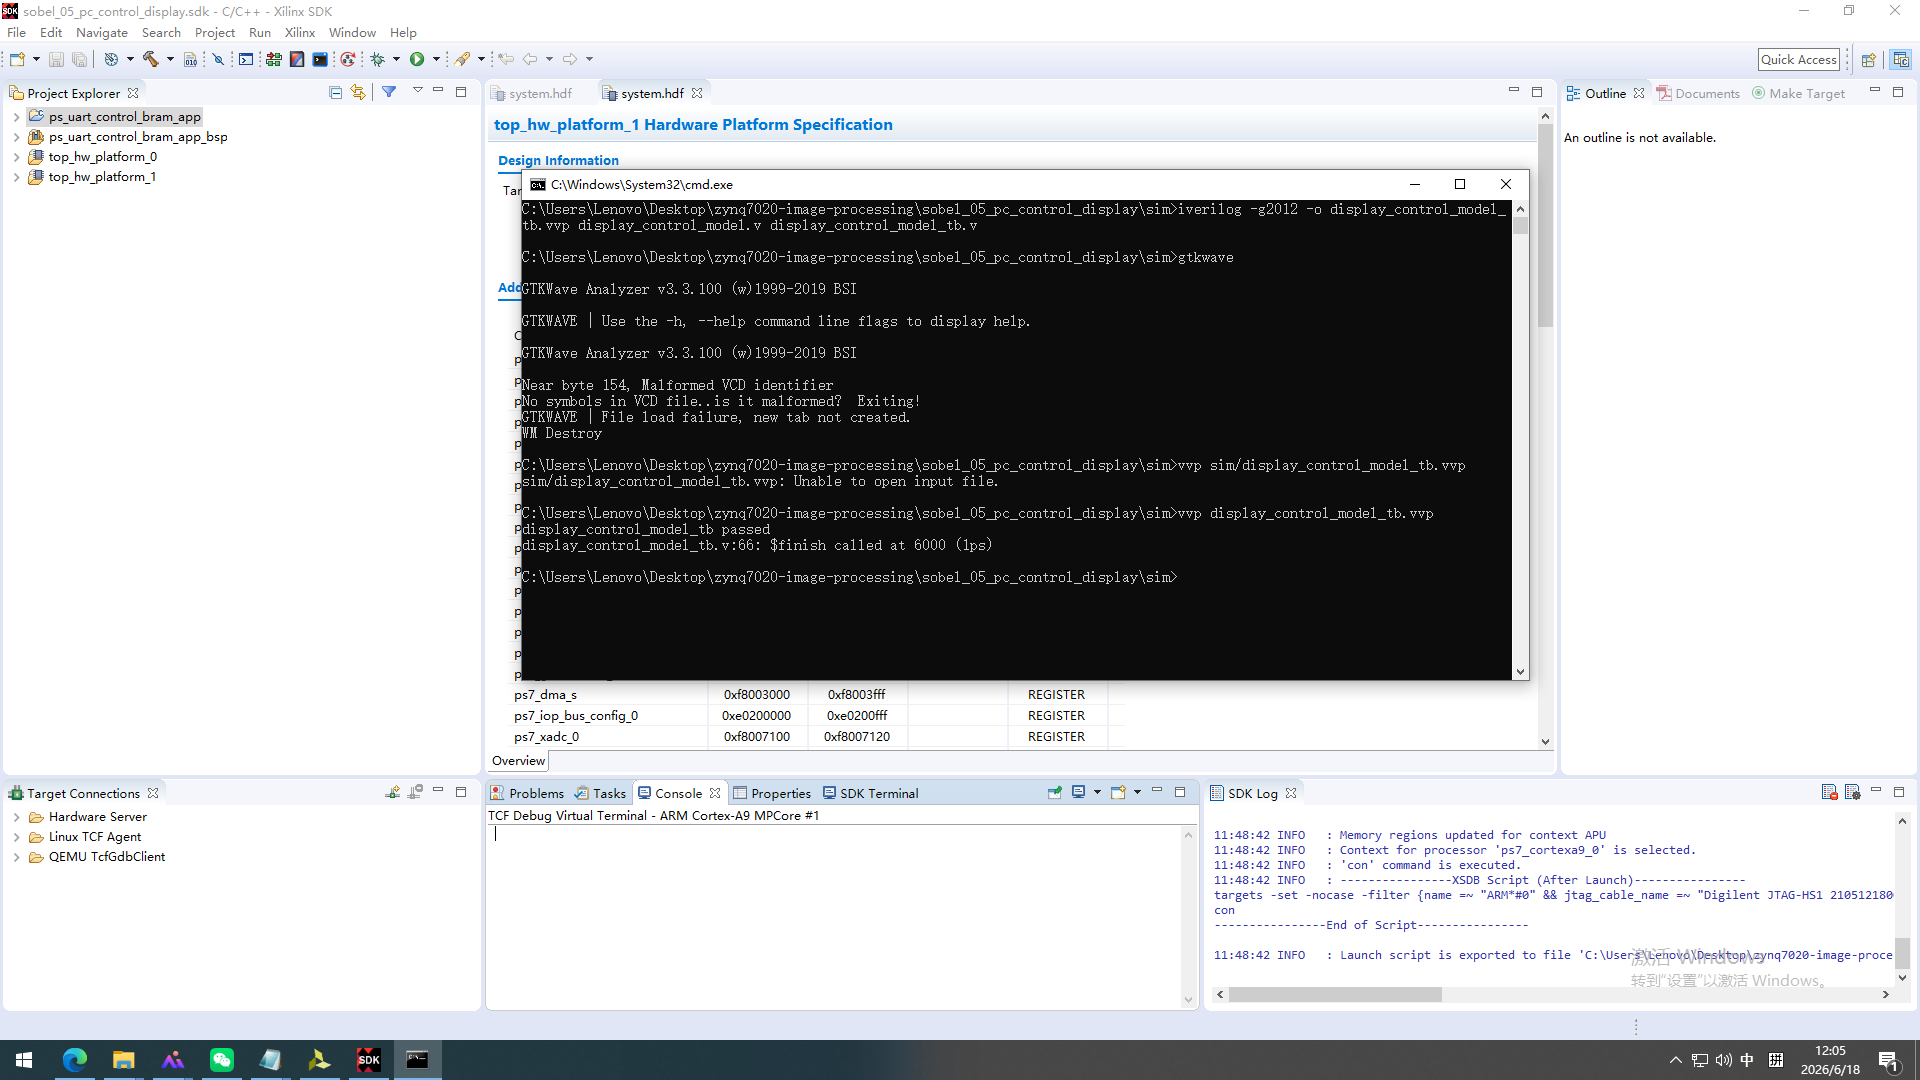
\includegraphics[width=0.9\textwidth]{images/05/仿真通过.png}
    \caption{显示控制模型仿真通过}
    \label{fig:sim_pass}
\end{figure}

如图\ref{fig:sim_pass}所示，仿真测试全部通过，验证了各模式下的显示逻辑正确性。

\begin{figure}[H]
    \centering
    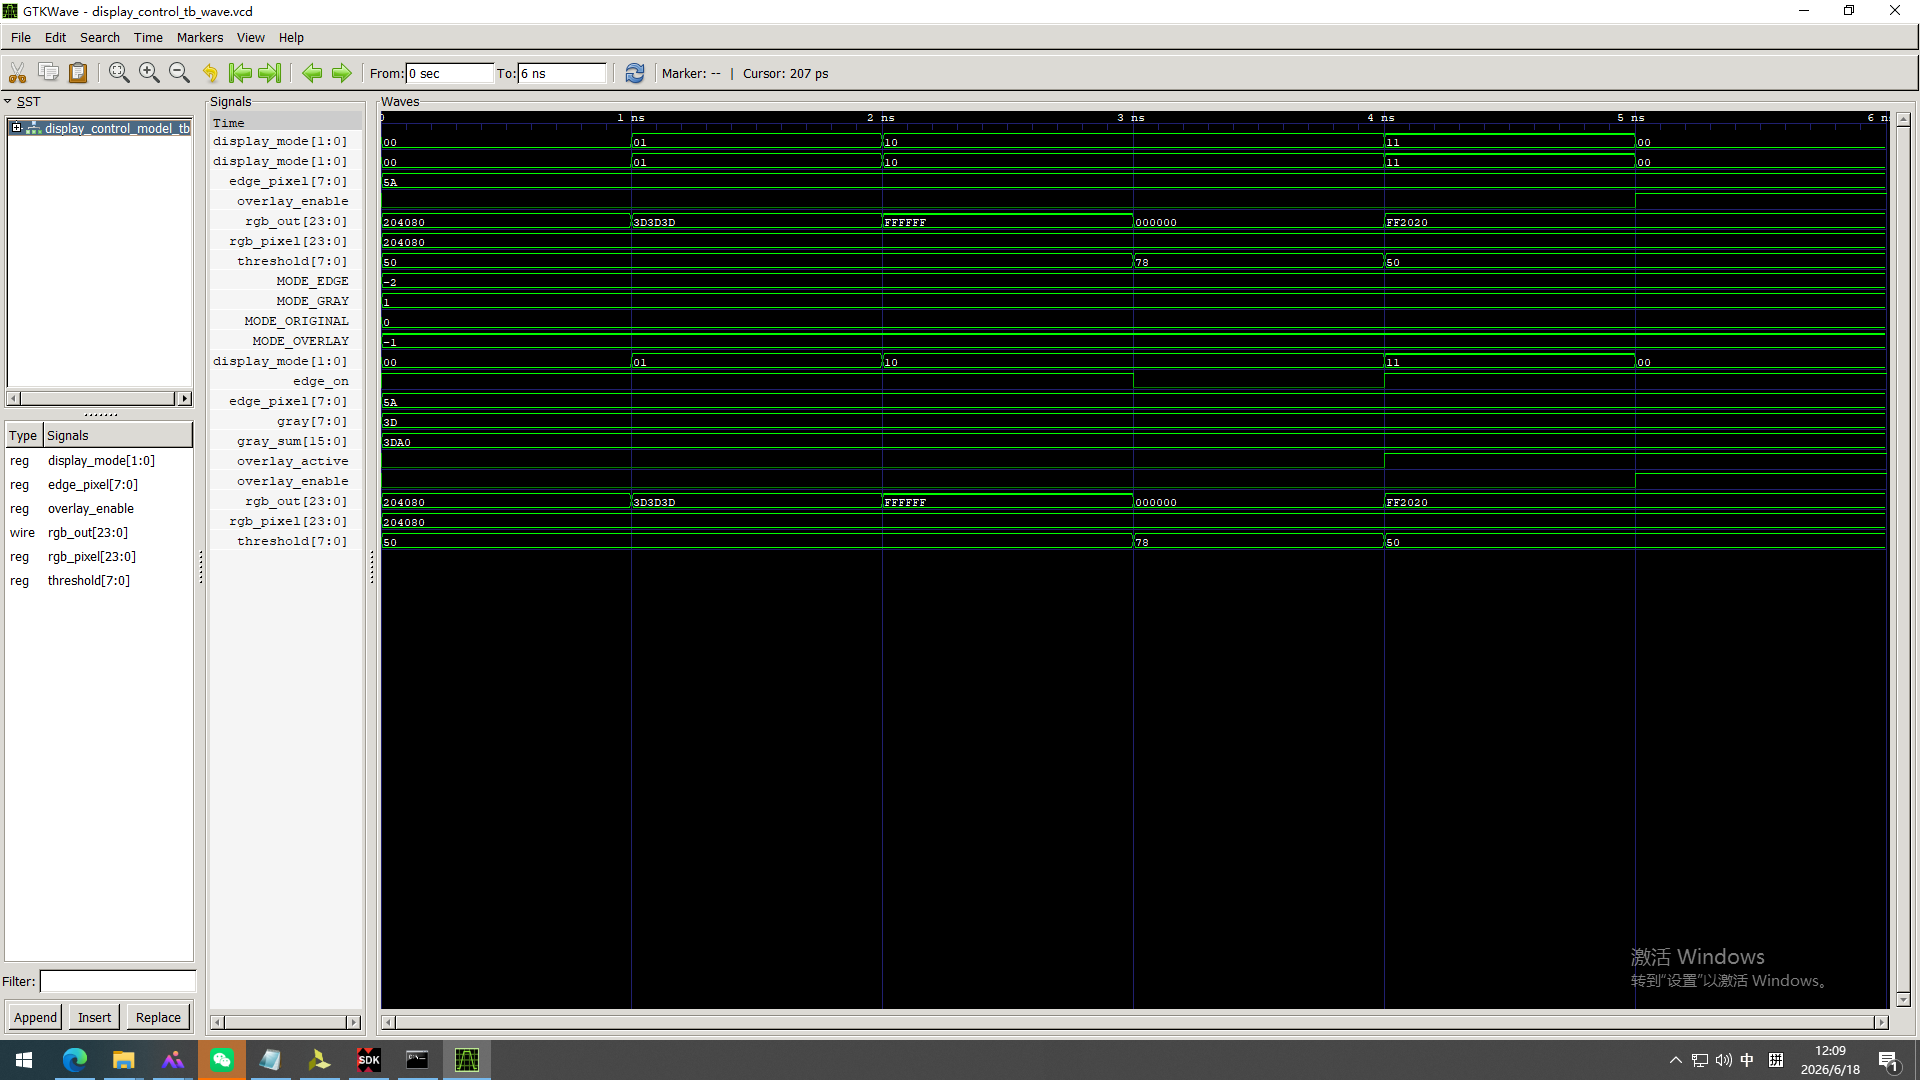
\includegraphics[width=0.9\textwidth]{images/05/仿真波形.png}
    \caption{显示控制模型仿真波形}
    \label{fig:sim_wave}
\end{figure}

如图\ref{fig:sim_wave}展示了关键信号的时序波形，包括display\_mode切换、edge\_data阈值比较和RGB输出。

\subsubsection{软件Golden Output对比}

使用Python生成4种算法的参考输出，对比如图\ref{fig:golden1}和\ref{fig:golden2}所示。

\begin{figure}[H]
    \centering
    \begin{minipage}{0.48\textwidth}
        \centering
        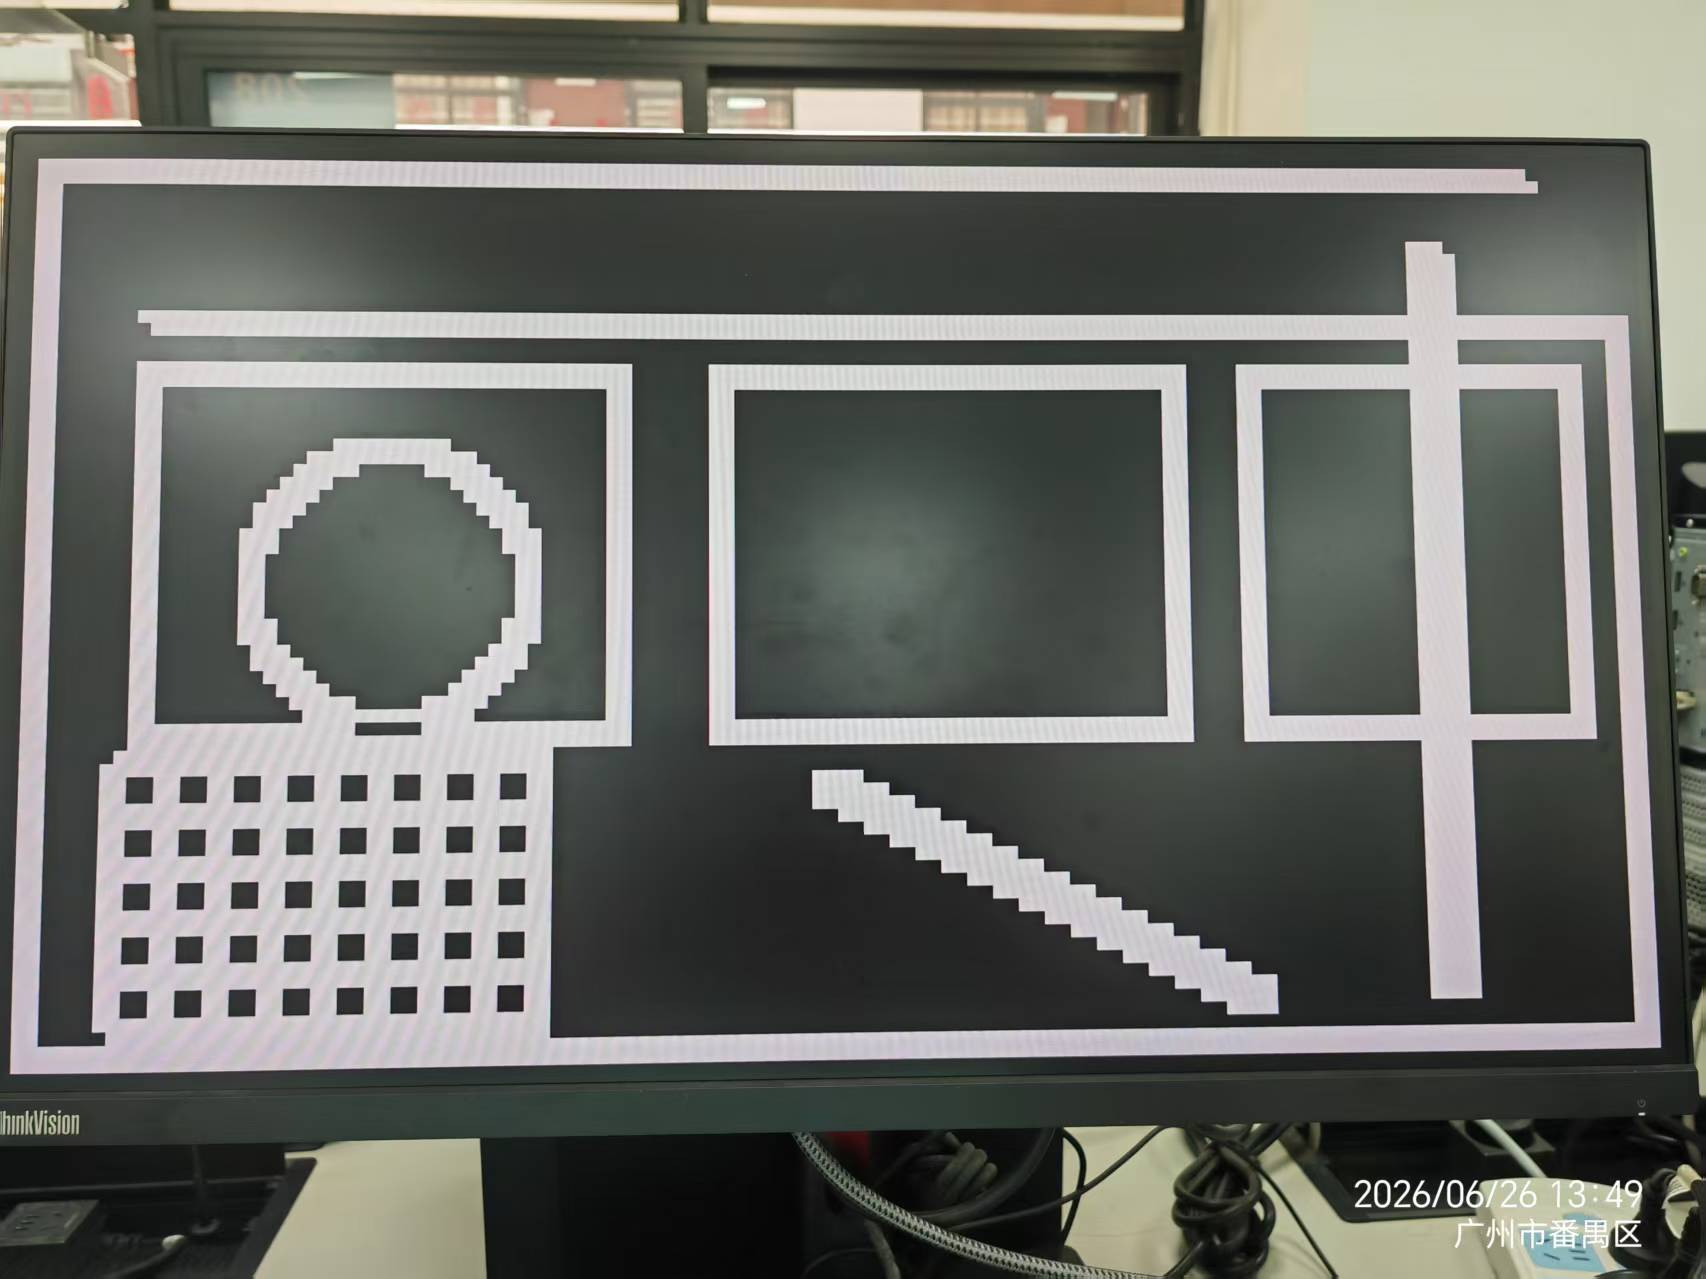
\includegraphics[width=\linewidth]{images/05扩展3/sobel_golden.jpg}
        \caption{Sobel}
    \end{minipage}
    \hfill
    \begin{minipage}{0.48\textwidth}
        \centering
        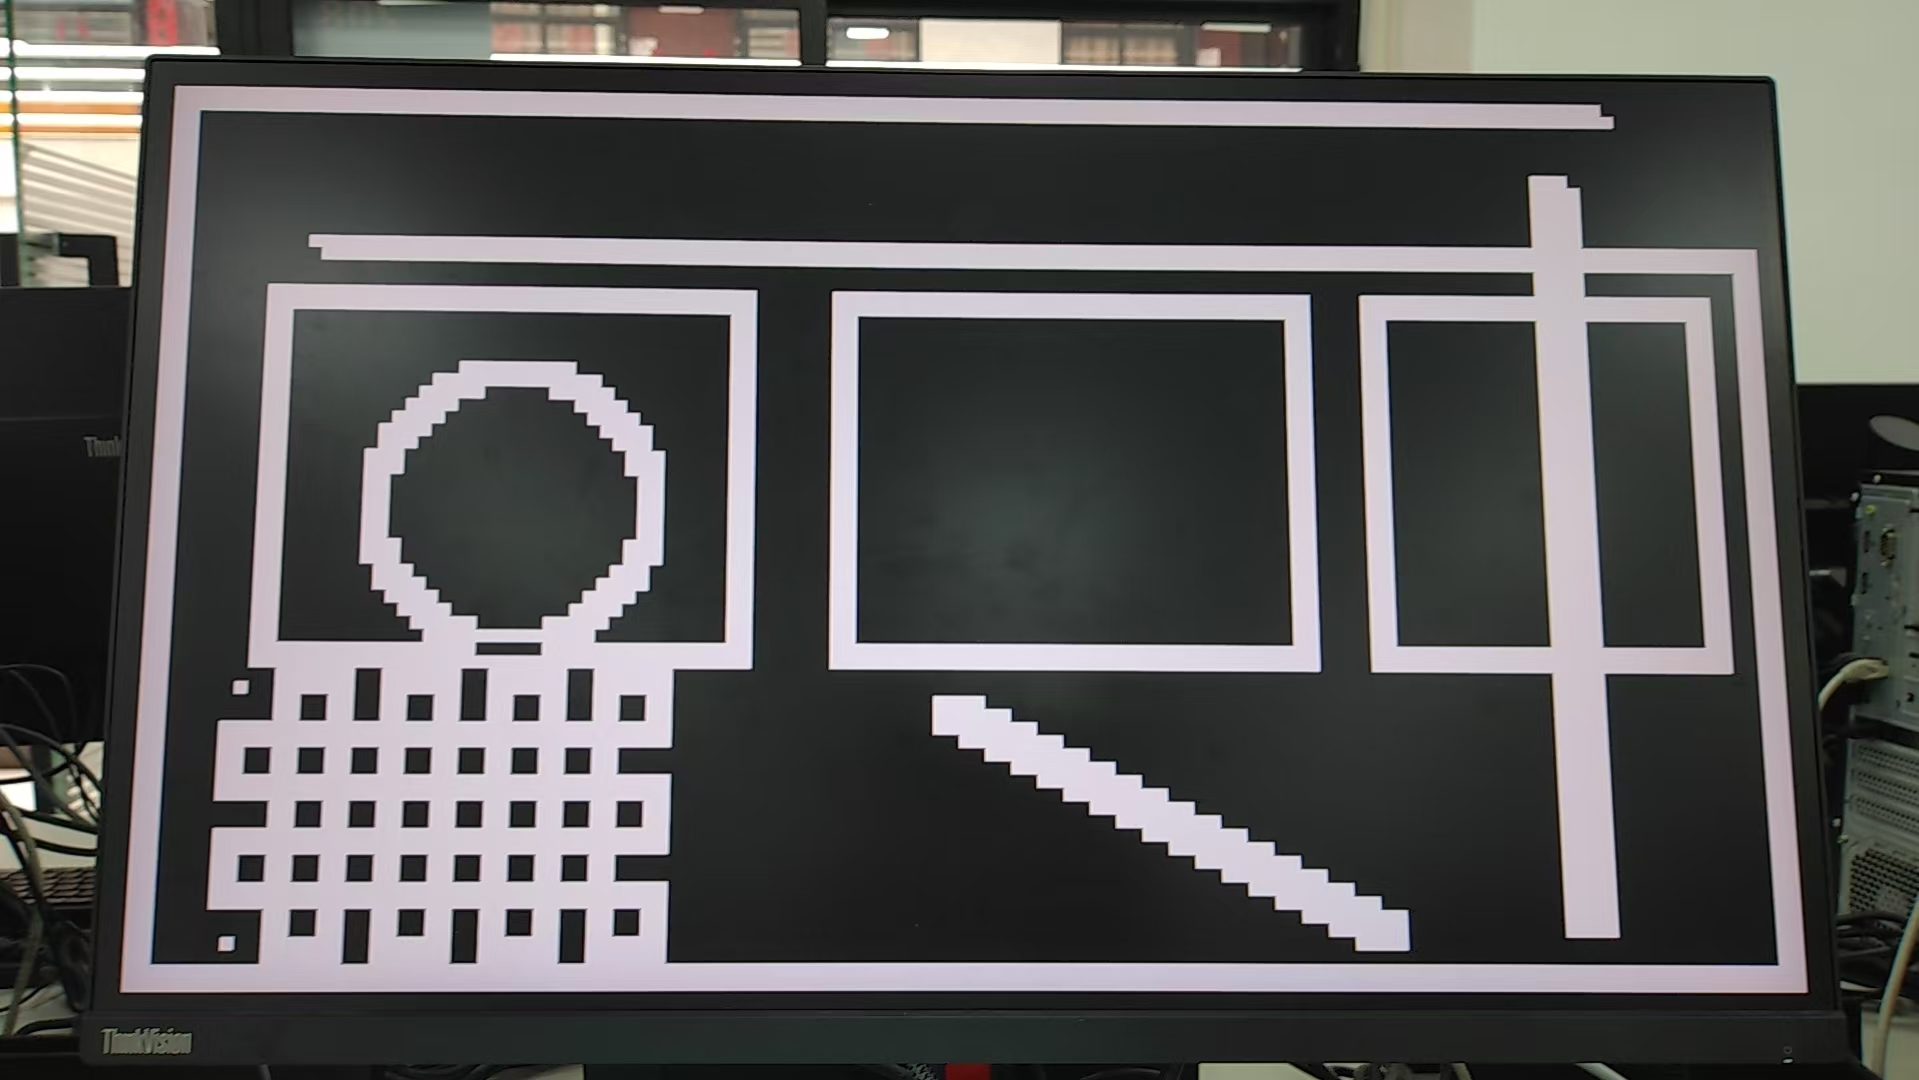
\includegraphics[width=\linewidth]{images/05扩展3/prewitt_golden.jpg}
        \caption{Prewitt}
    \end{minipage}
    \caption{Sobel与Prewitt Golden Output对比}
    \label{fig:golden1}
\end{figure}

从图\ref{fig:golden1}中可以观察到：Sobel算法边缘响应最均衡，对水平和垂直边缘都有较好的检测效果；Prewitt算法由于去掉了2x中心权重，边缘响应整体较弱，但边缘更平滑。

\begin{figure}[H]
    \centering
    \begin{minipage}{0.48\textwidth}
        \centering
        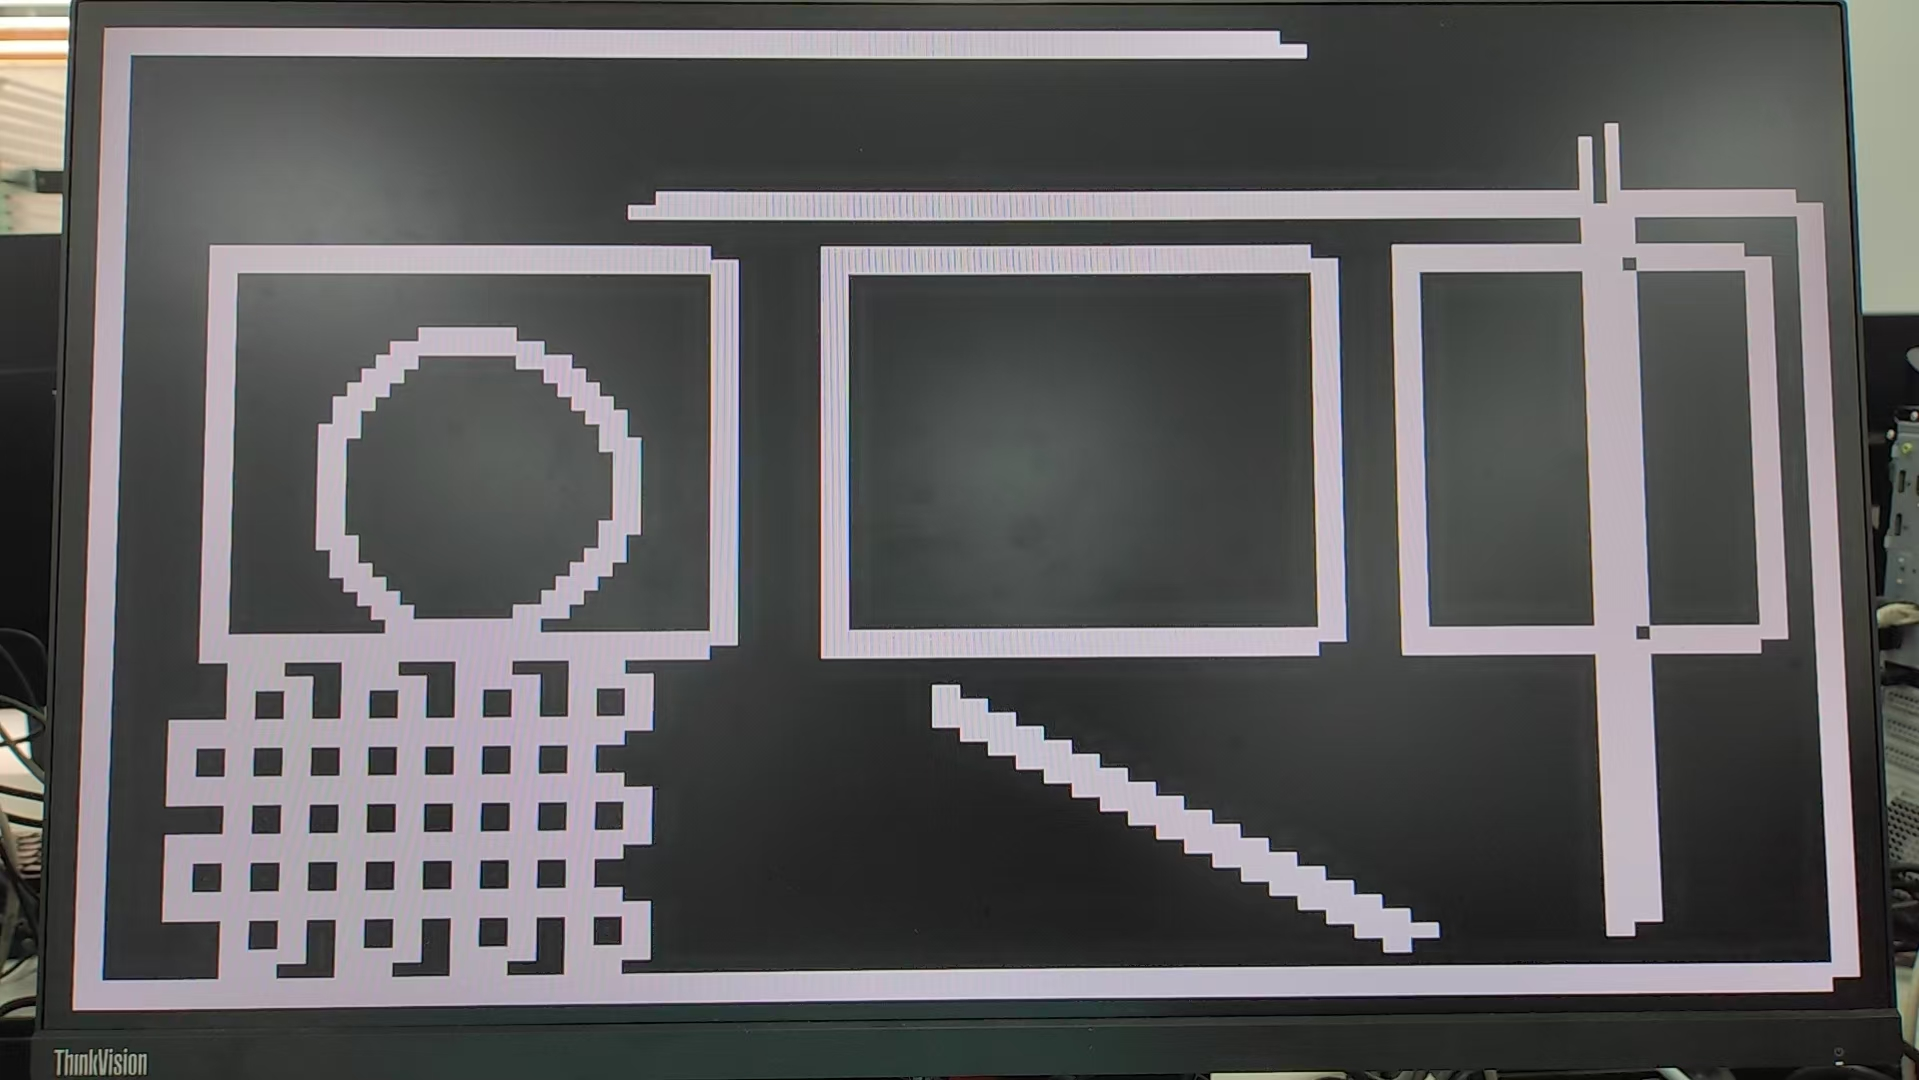
\includegraphics[width=\linewidth]{images/05扩展3/laplacian_golden.jpg}
        \caption{Laplacian}
    \end{minipage}
    \hfill
    \begin{minipage}{0.48\textwidth}
        \centering
        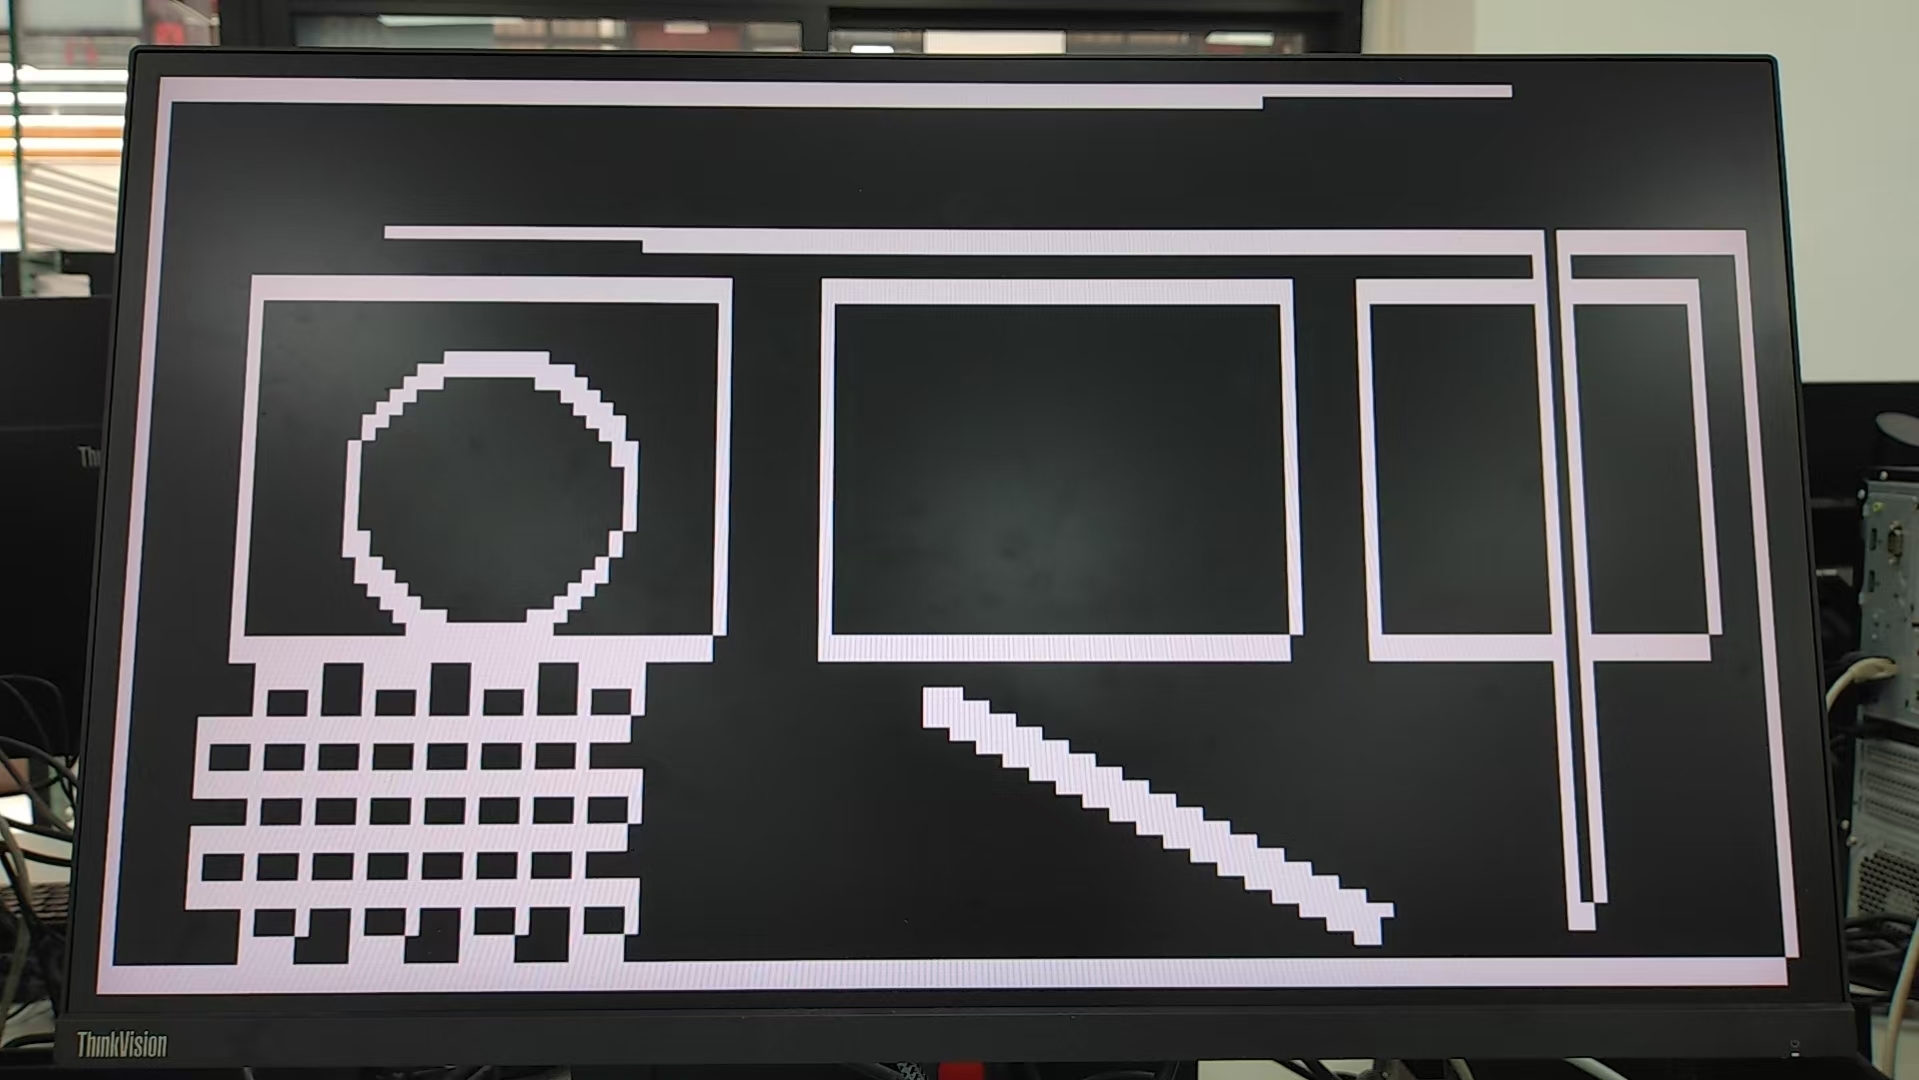
\includegraphics[width=\linewidth]{images/05扩展3/Robert_golden.jpg}
        \caption{Roberts}
    \end{minipage}
    \caption{Laplacian与Roberts Golden Output对比}
    \label{fig:golden2}
\end{figure}

从图\ref{fig:golden2}中可以观察到：Laplacian作为二阶导数算子，边缘细节最丰富，但对噪声也更敏感；Roberts使用2×2小卷积核，边缘响应较强，适合检测对角线方向的边缘。

\subsubsection{不同阈值对比}

在阈值40、60、80下对比四种算法的边缘检测结果。

\begin{figure}[H]
    \centering
    \begin{minipage}{0.48\textwidth}
        \centering
        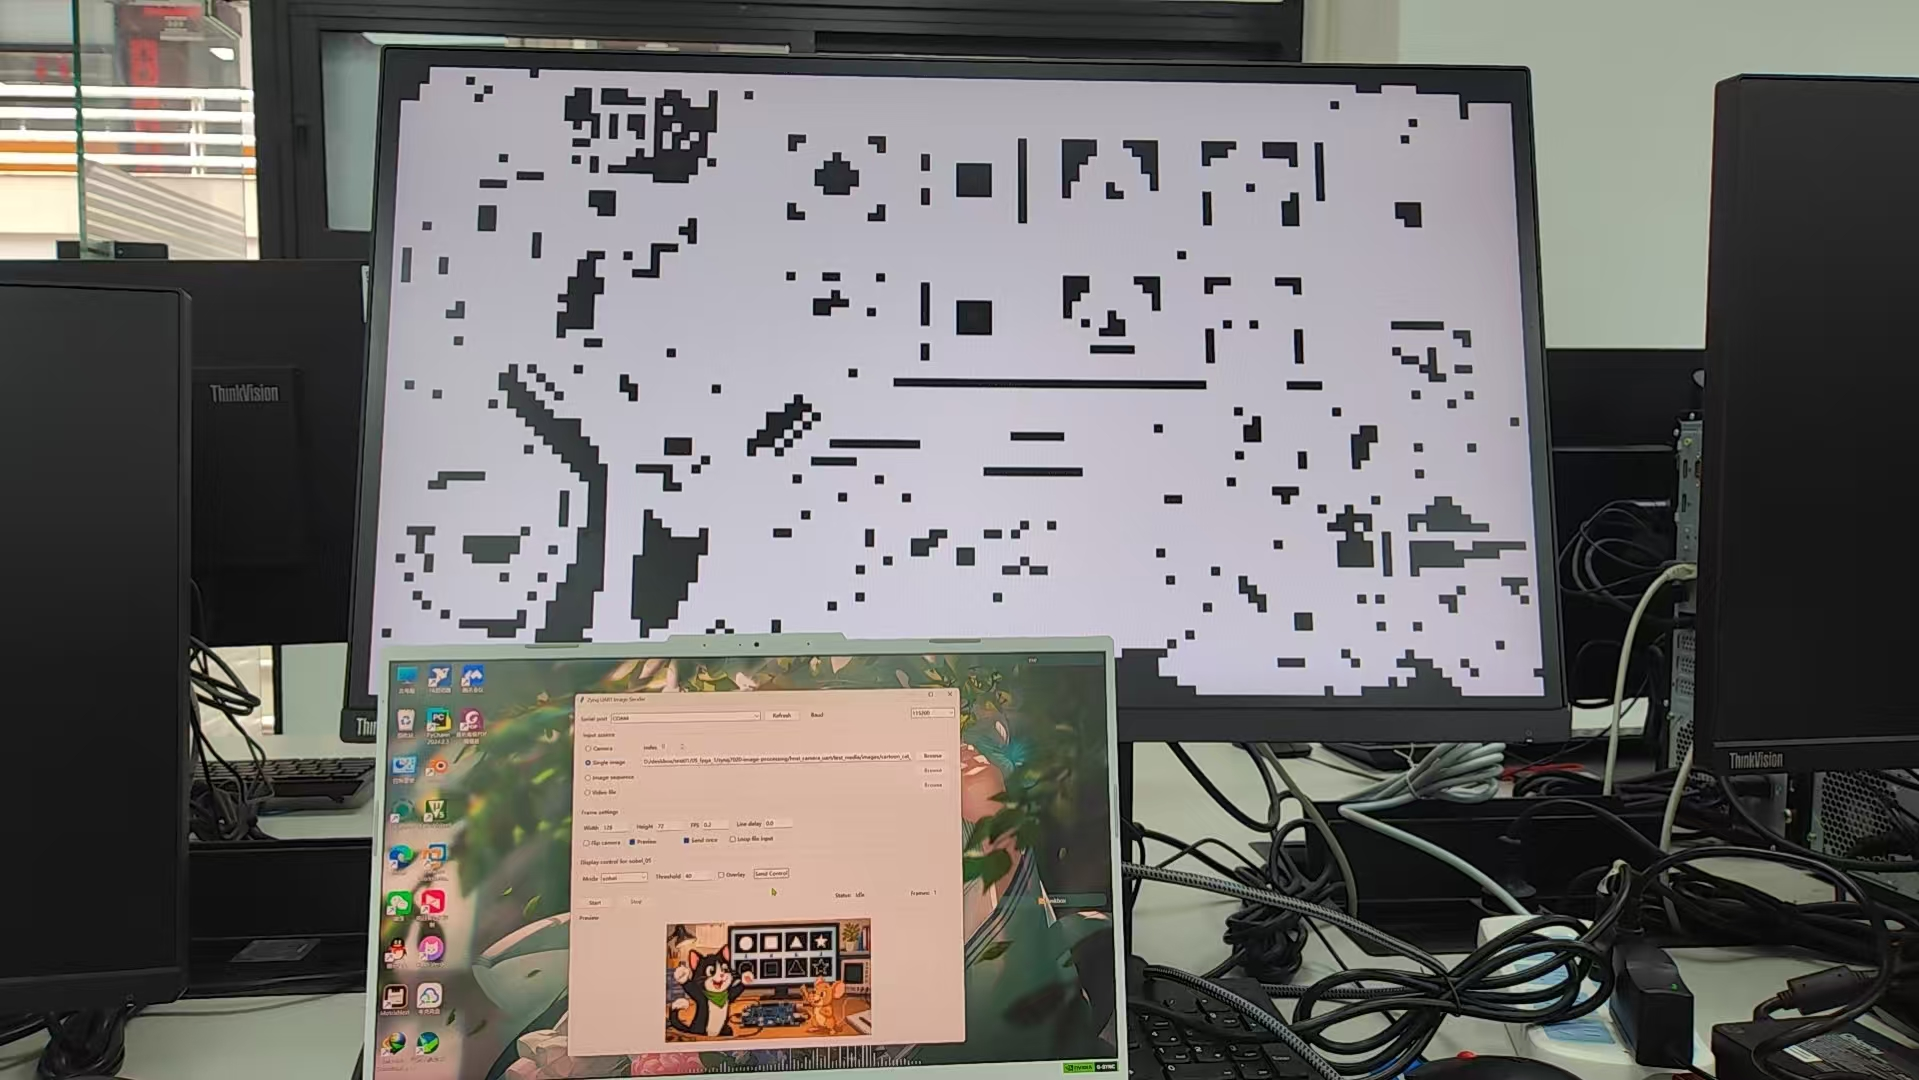
\includegraphics[width=\linewidth]{images/05扩展3/sobel_40.jpg}
        \caption{Sobel}
    \end{minipage}
    \hfill
    \begin{minipage}{0.48\textwidth}
        \centering
        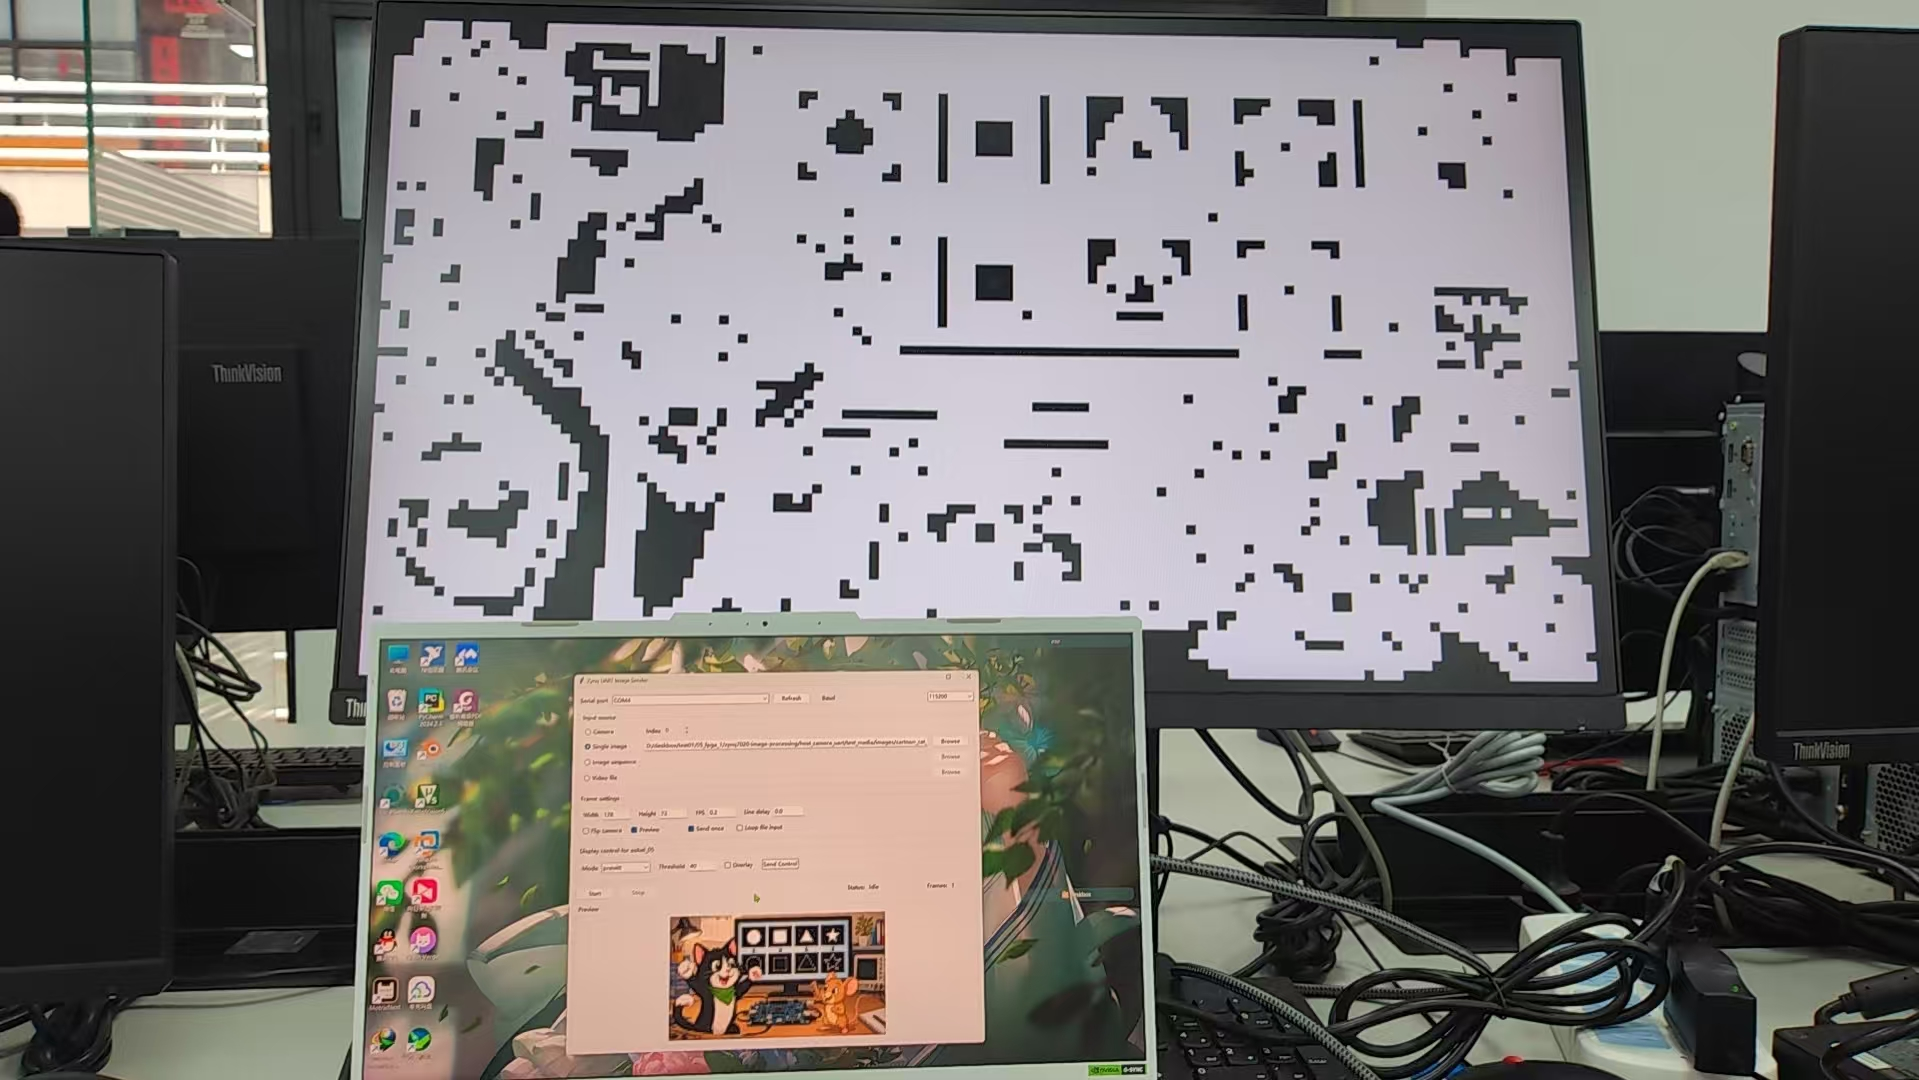
\includegraphics[width=\linewidth]{images/05扩展3/prewitt_40.jpg}
        \caption{Prewitt}
    \end{minipage}
    \par\vspace{1em}
    \begin{minipage}{0.48\textwidth}
        \centering
        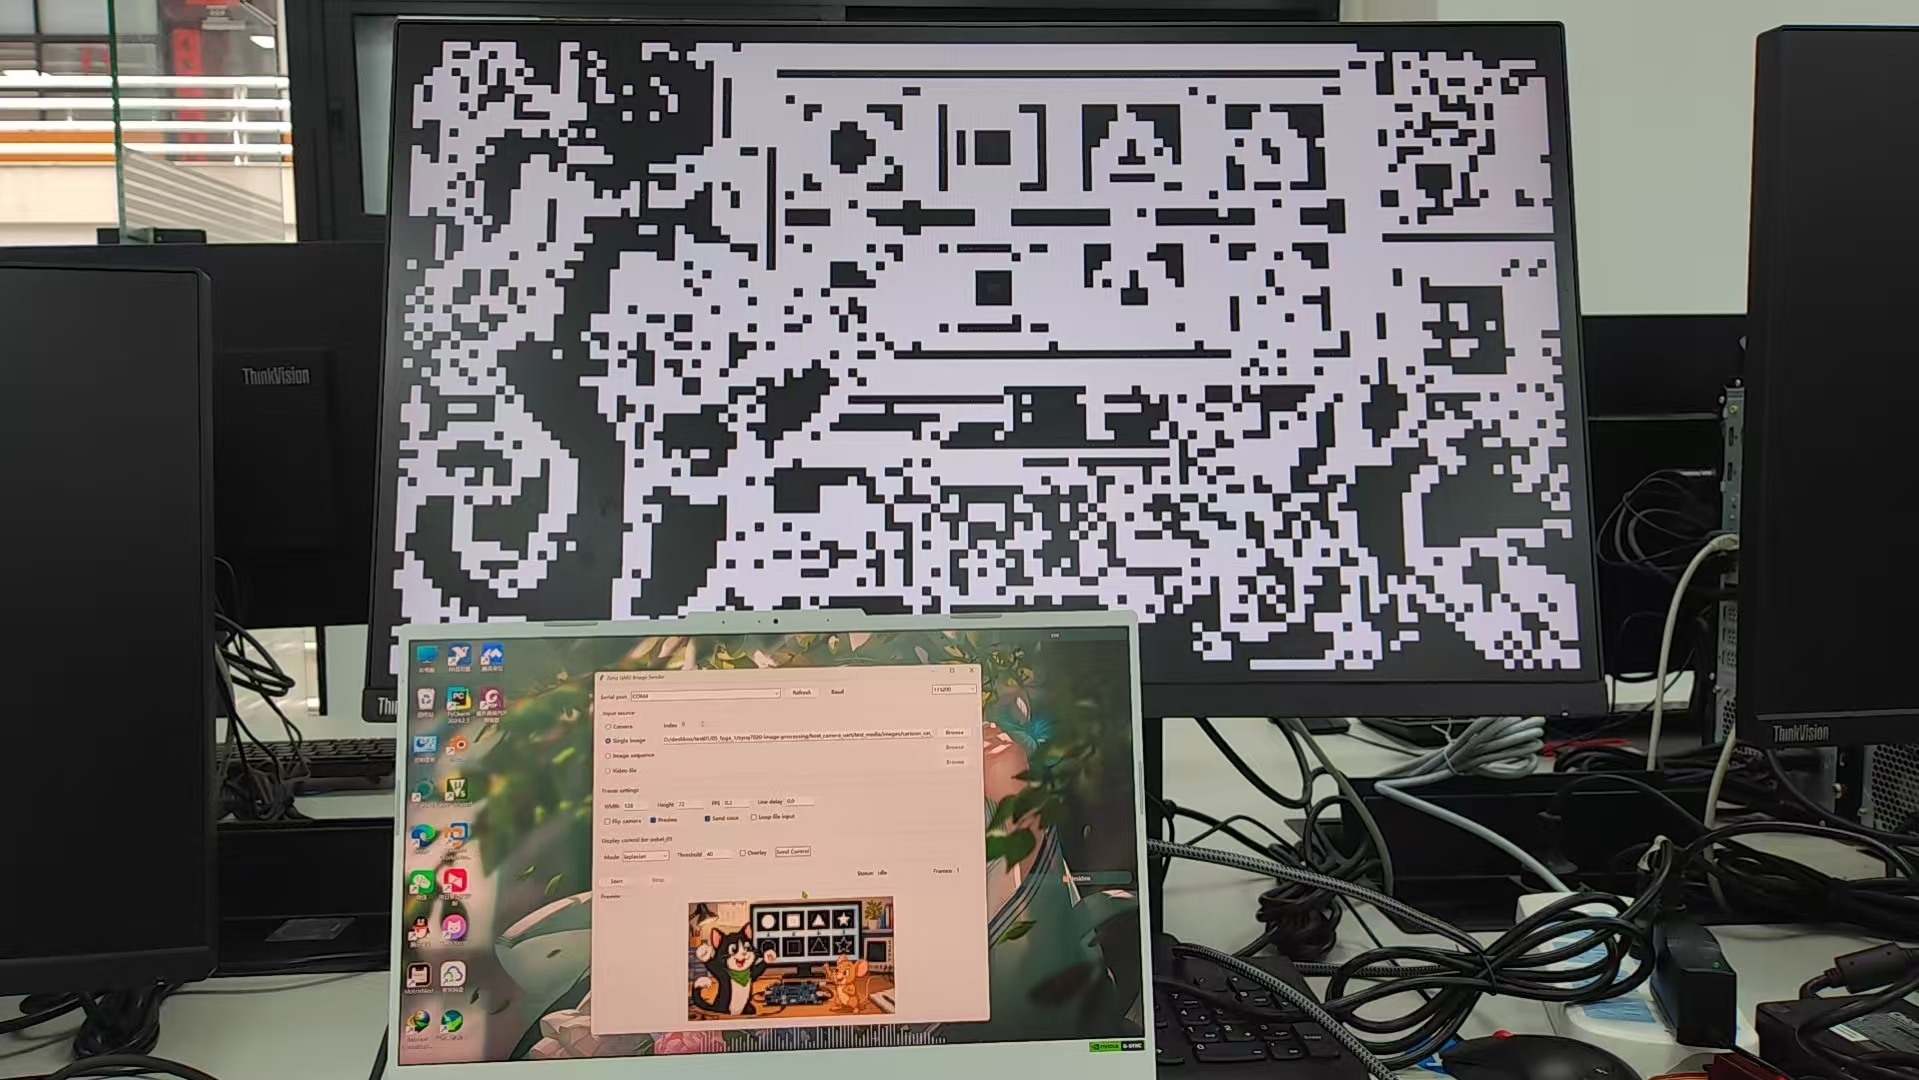
\includegraphics[width=\linewidth]{images/05扩展3/laplacian_40.jpg}
        \caption{Laplacian}
    \end{minipage}
    \hfill
    \begin{minipage}{0.48\textwidth}
        \centering
        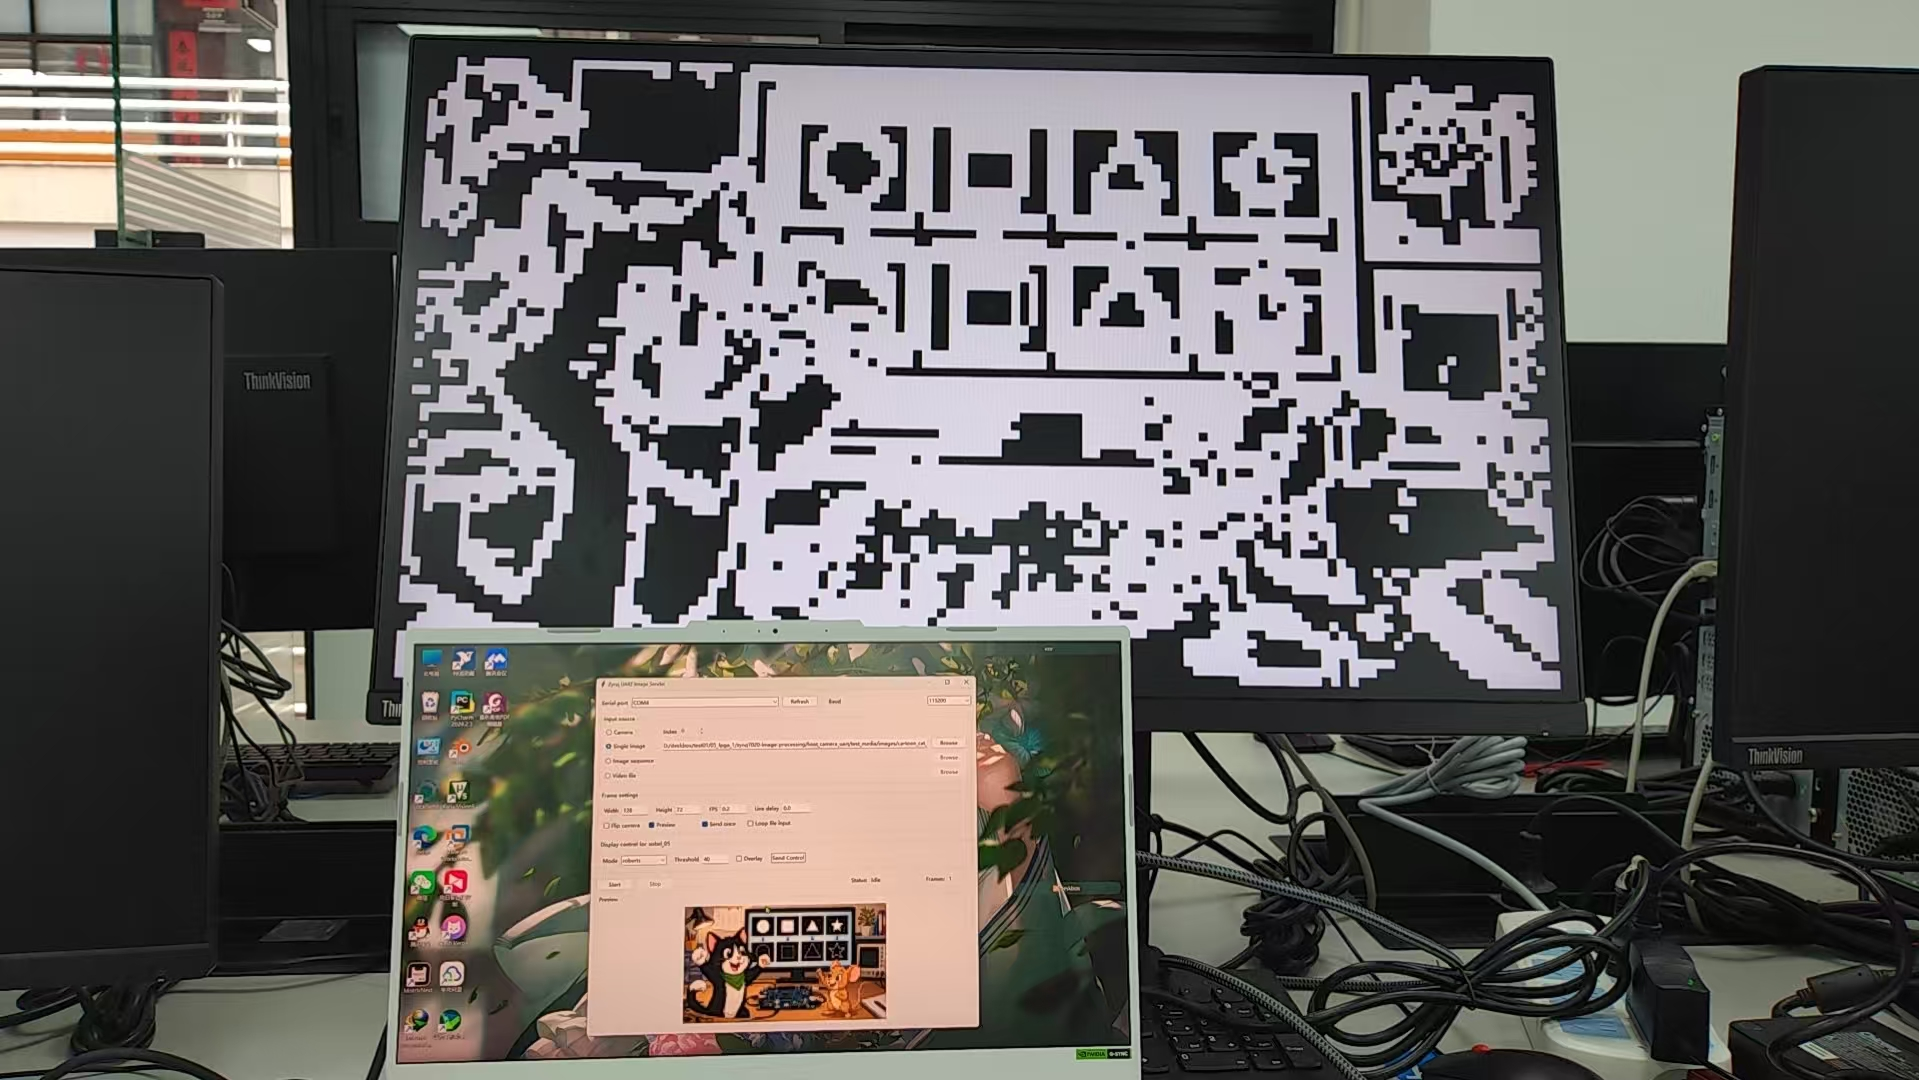
\includegraphics[width=\linewidth]{images/05扩展3/Robert_40.jpg}
        \caption{Roberts}
    \end{minipage}
    \caption{阈值40时四种算法对比}
    \label{fig:thresh40}
\end{figure}

如图\ref{fig:thresh40}所示，当阈值为40时，四种算法都检测到较多边缘。Sobel和Prewitt的边缘效果较为均衡，适合通用场景；Laplacian的边缘细节最丰富，但噪点也最多；Roberts的边缘响应较强，适合检测对角线方向的边缘。

\begin{figure}[H]
    \centering
    \begin{minipage}{0.48\textwidth}
        \centering
        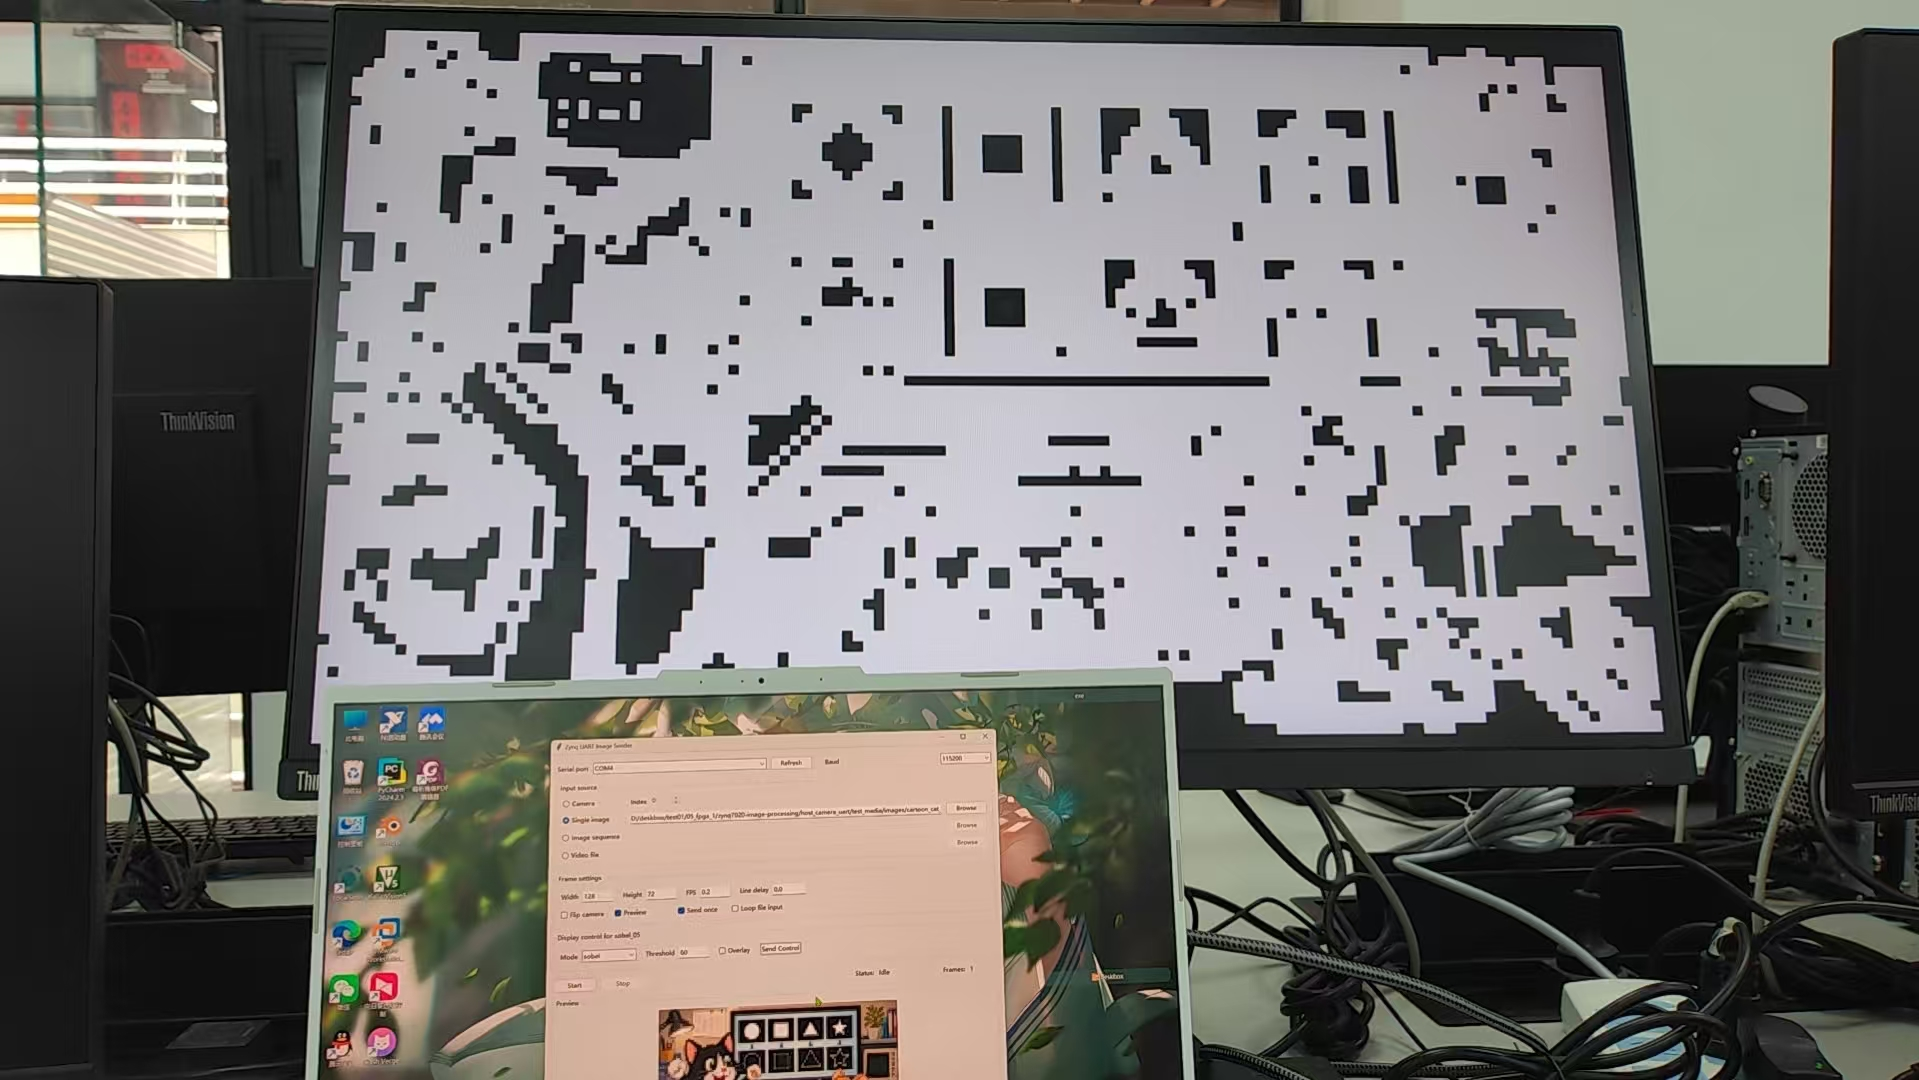
\includegraphics[width=\linewidth]{images/05扩展3/sobel_60.jpg}
        \caption{Sobel}
    \end{minipage}
    \hfill
    \begin{minipage}{0.48\textwidth}
        \centering
        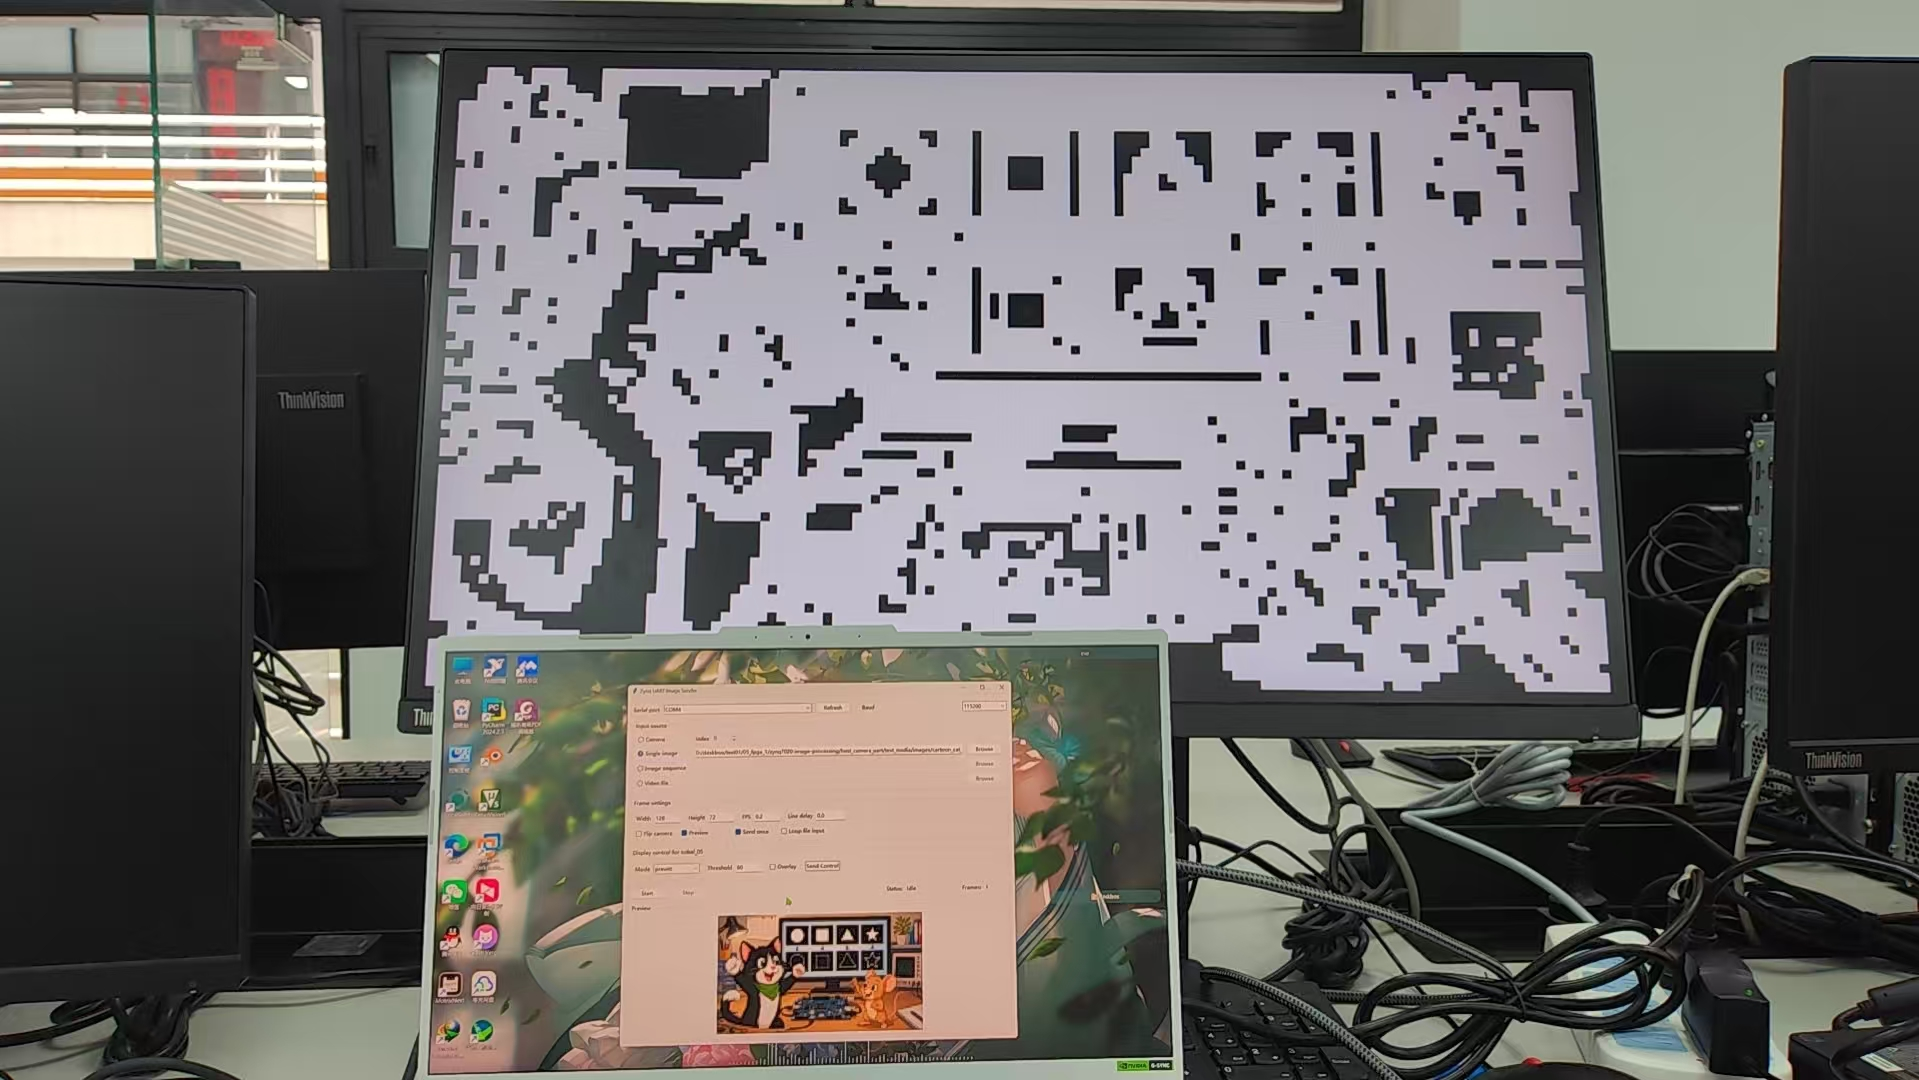
\includegraphics[width=\linewidth]{images/05扩展3/prewitt_60.jpg}
        \caption{Prewitt}
    \end{minipage}
    \par\vspace{1em}
    \begin{minipage}{0.48\textwidth}
        \centering
        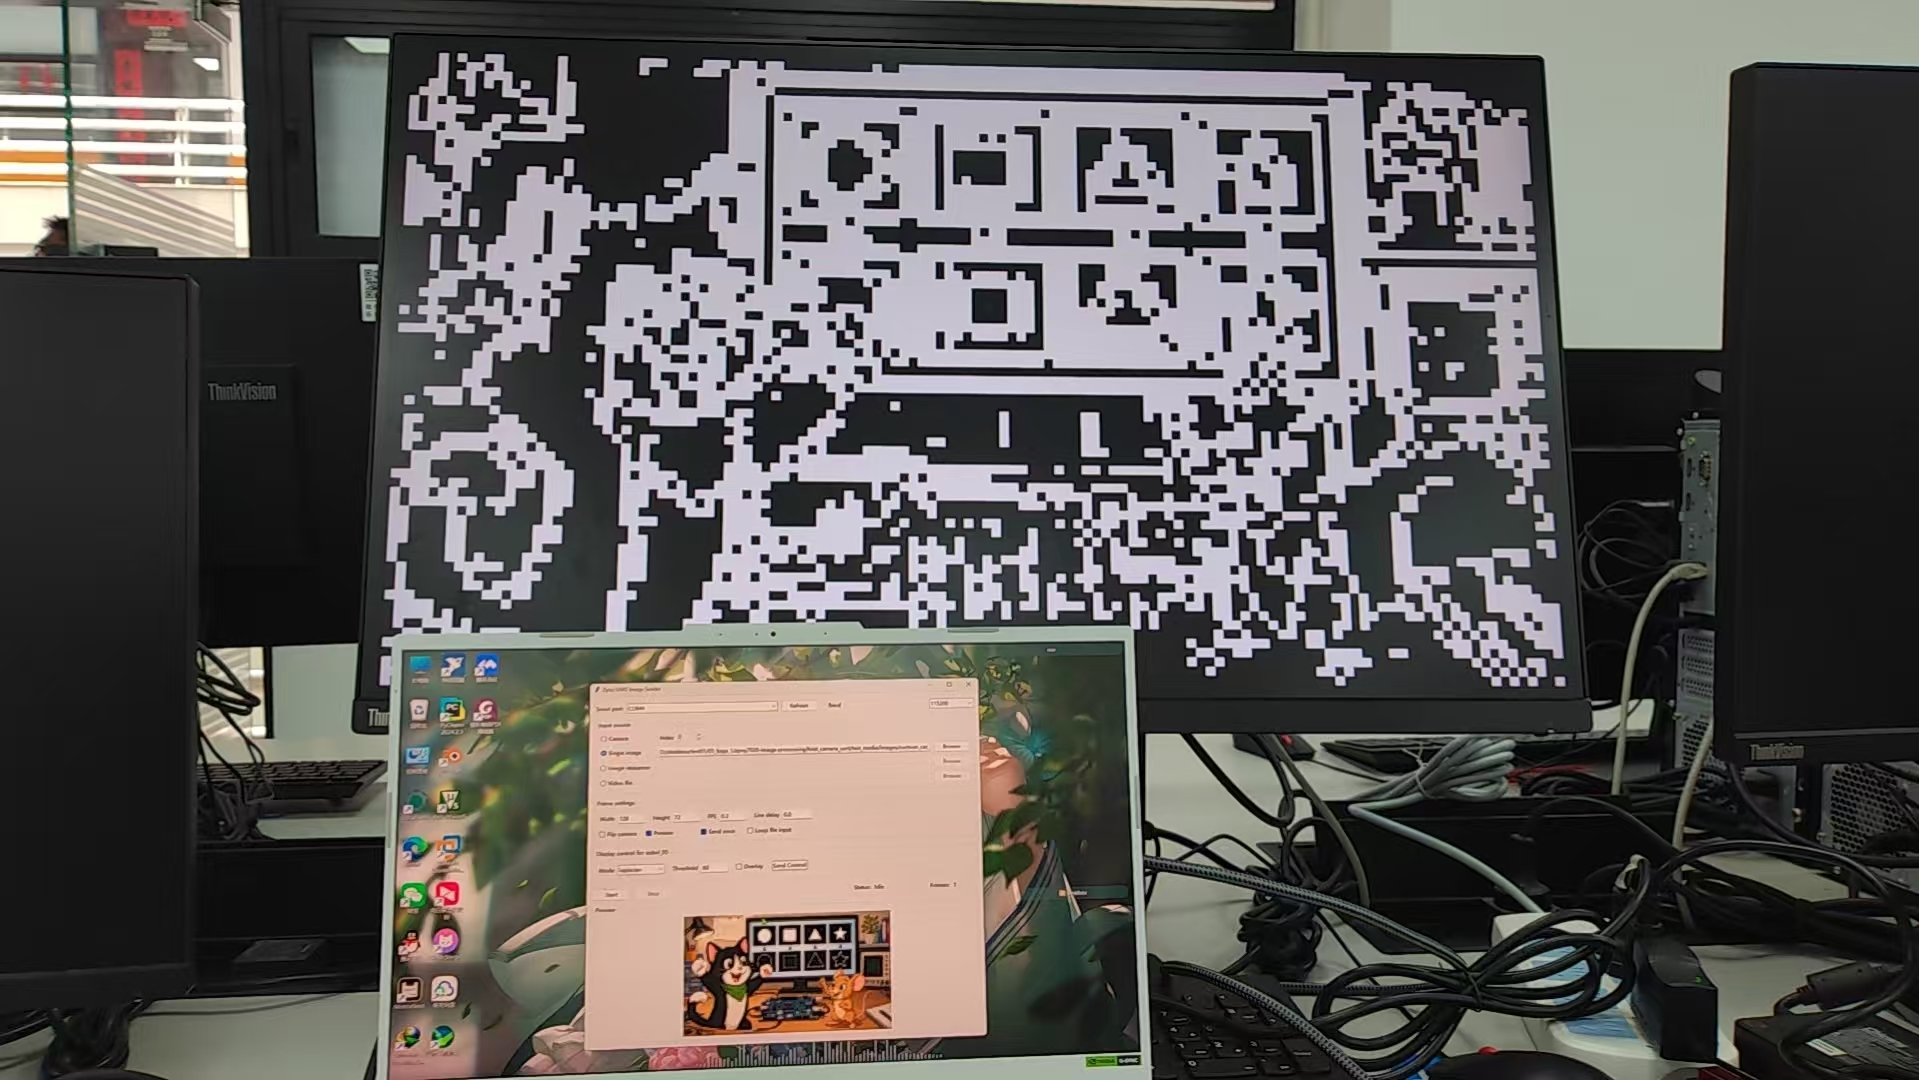
\includegraphics[width=\linewidth]{images/05扩展3/laplacian_60.jpg}
        \caption{Laplacian}
    \end{minipage}
    \hfill
    \begin{minipage}{0.48\textwidth}
        \centering
        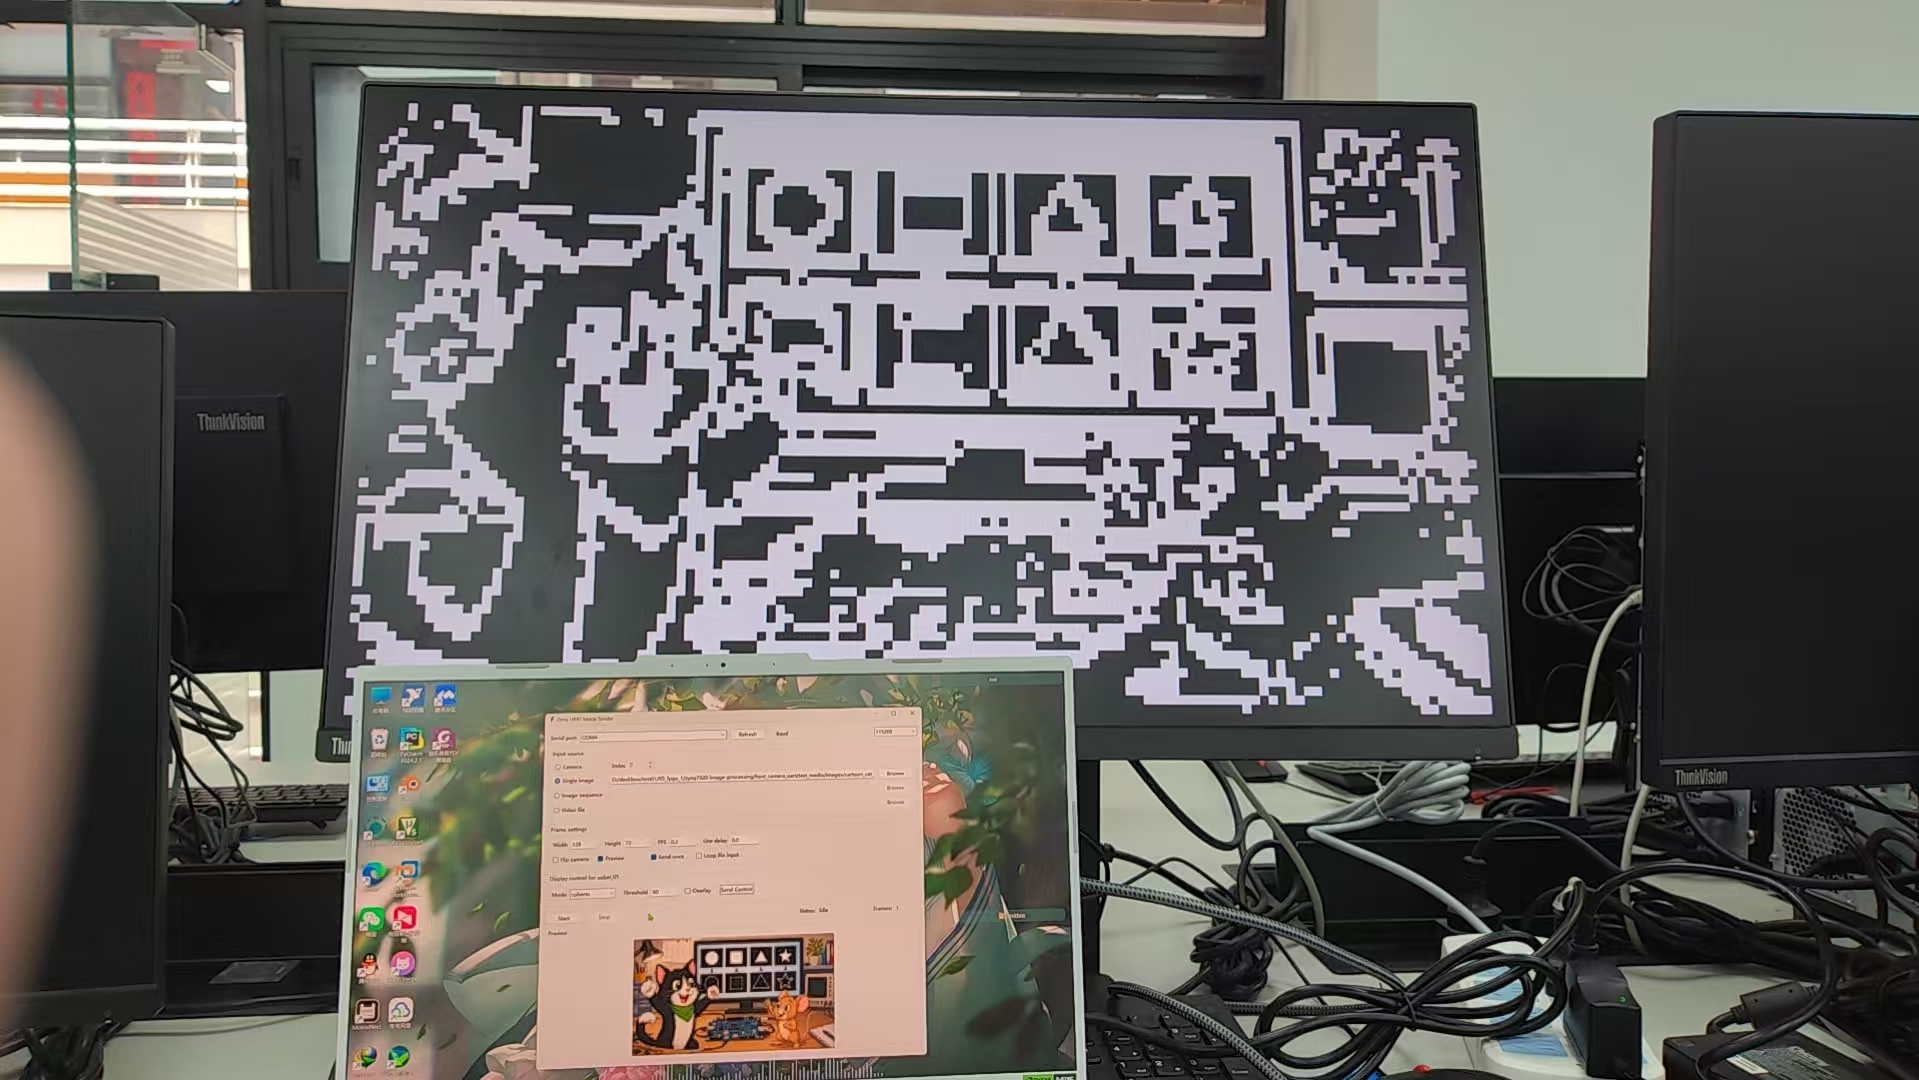
\includegraphics[width=\linewidth]{images/05扩展3/Robert_60.jpg}
        \caption{Roberts}
    \end{minipage}
    \caption{阈值60时四种算法对比}
    \label{fig:thresh60}
\end{figure}

如图\ref{fig:thresh60}所示，当阈值提高到60时，各算法检测到的边缘减少，噪声得到一定抑制。Sobel和Prewitt的边缘更加清晰，Laplacian的噪点有所减少但仍比其他算法多。这说明提高阈值可以有效抑制噪声，但也会丢失一些弱边缘信息。

\begin{figure}[H]
    \centering
    \begin{minipage}{0.48\textwidth}
        \centering
        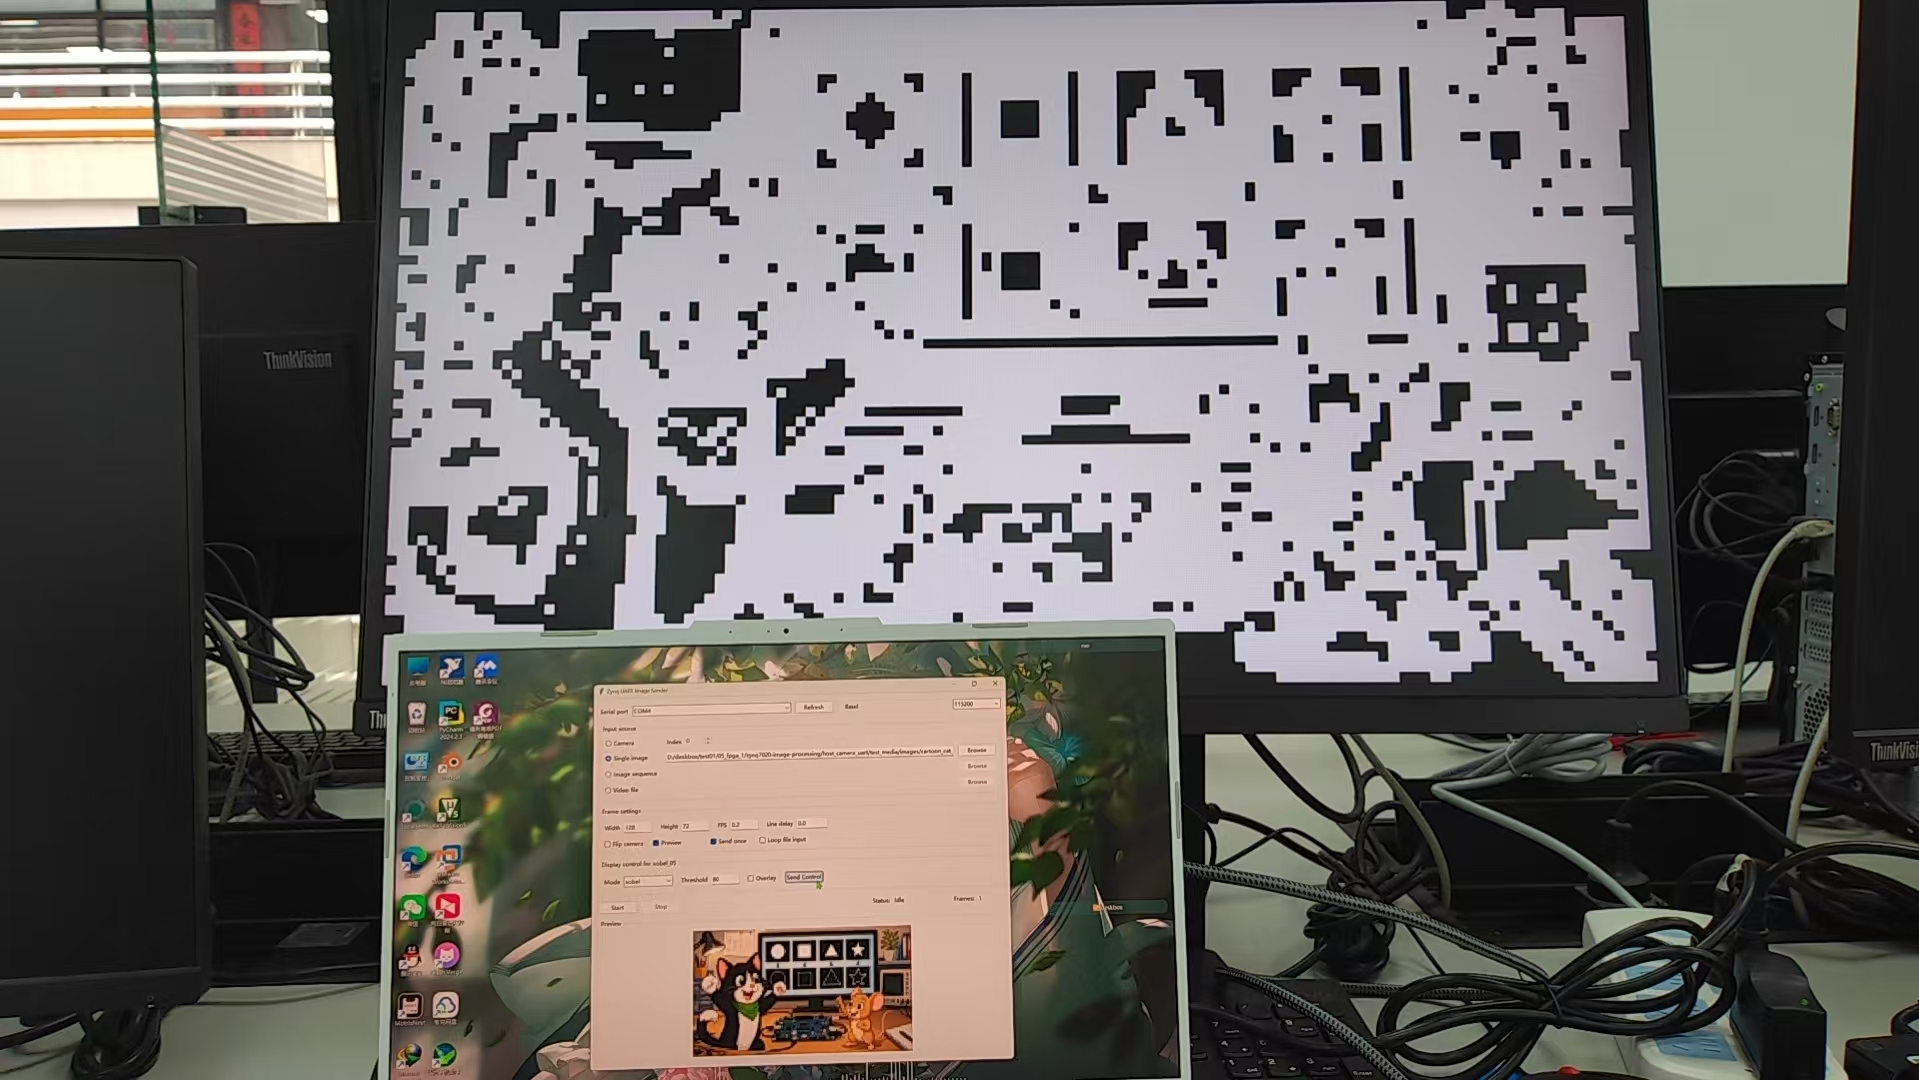
\includegraphics[width=\linewidth]{images/05扩展3/sobel_80.jpg}
        \caption{Sobel}
    \end{minipage}
    \hfill
    \begin{minipage}{0.48\textwidth}
        \centering
        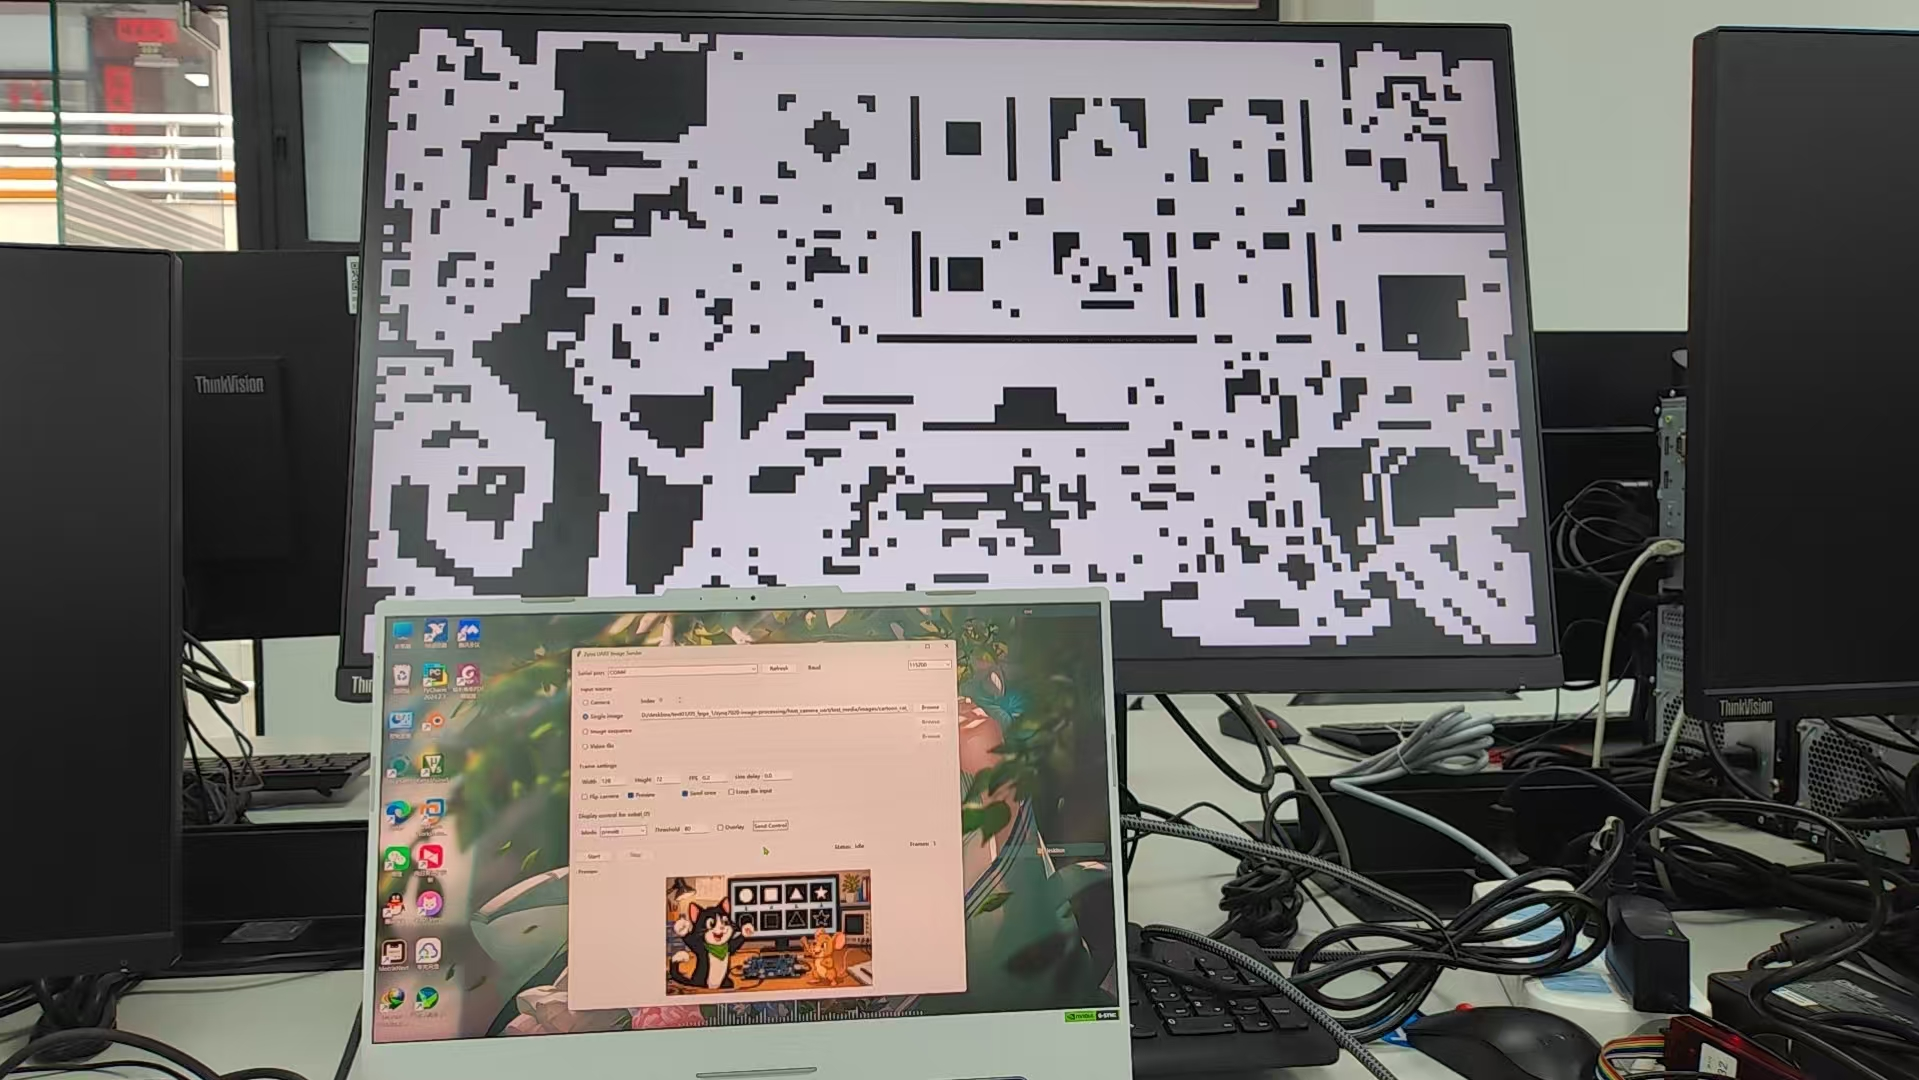
\includegraphics[width=\linewidth]{images/05扩展3/prewitt_80.jpg}
        \caption{Prewitt}
    \end{minipage}
    \par\vspace{1em}
    \begin{minipage}{0.48\textwidth}
        \centering
        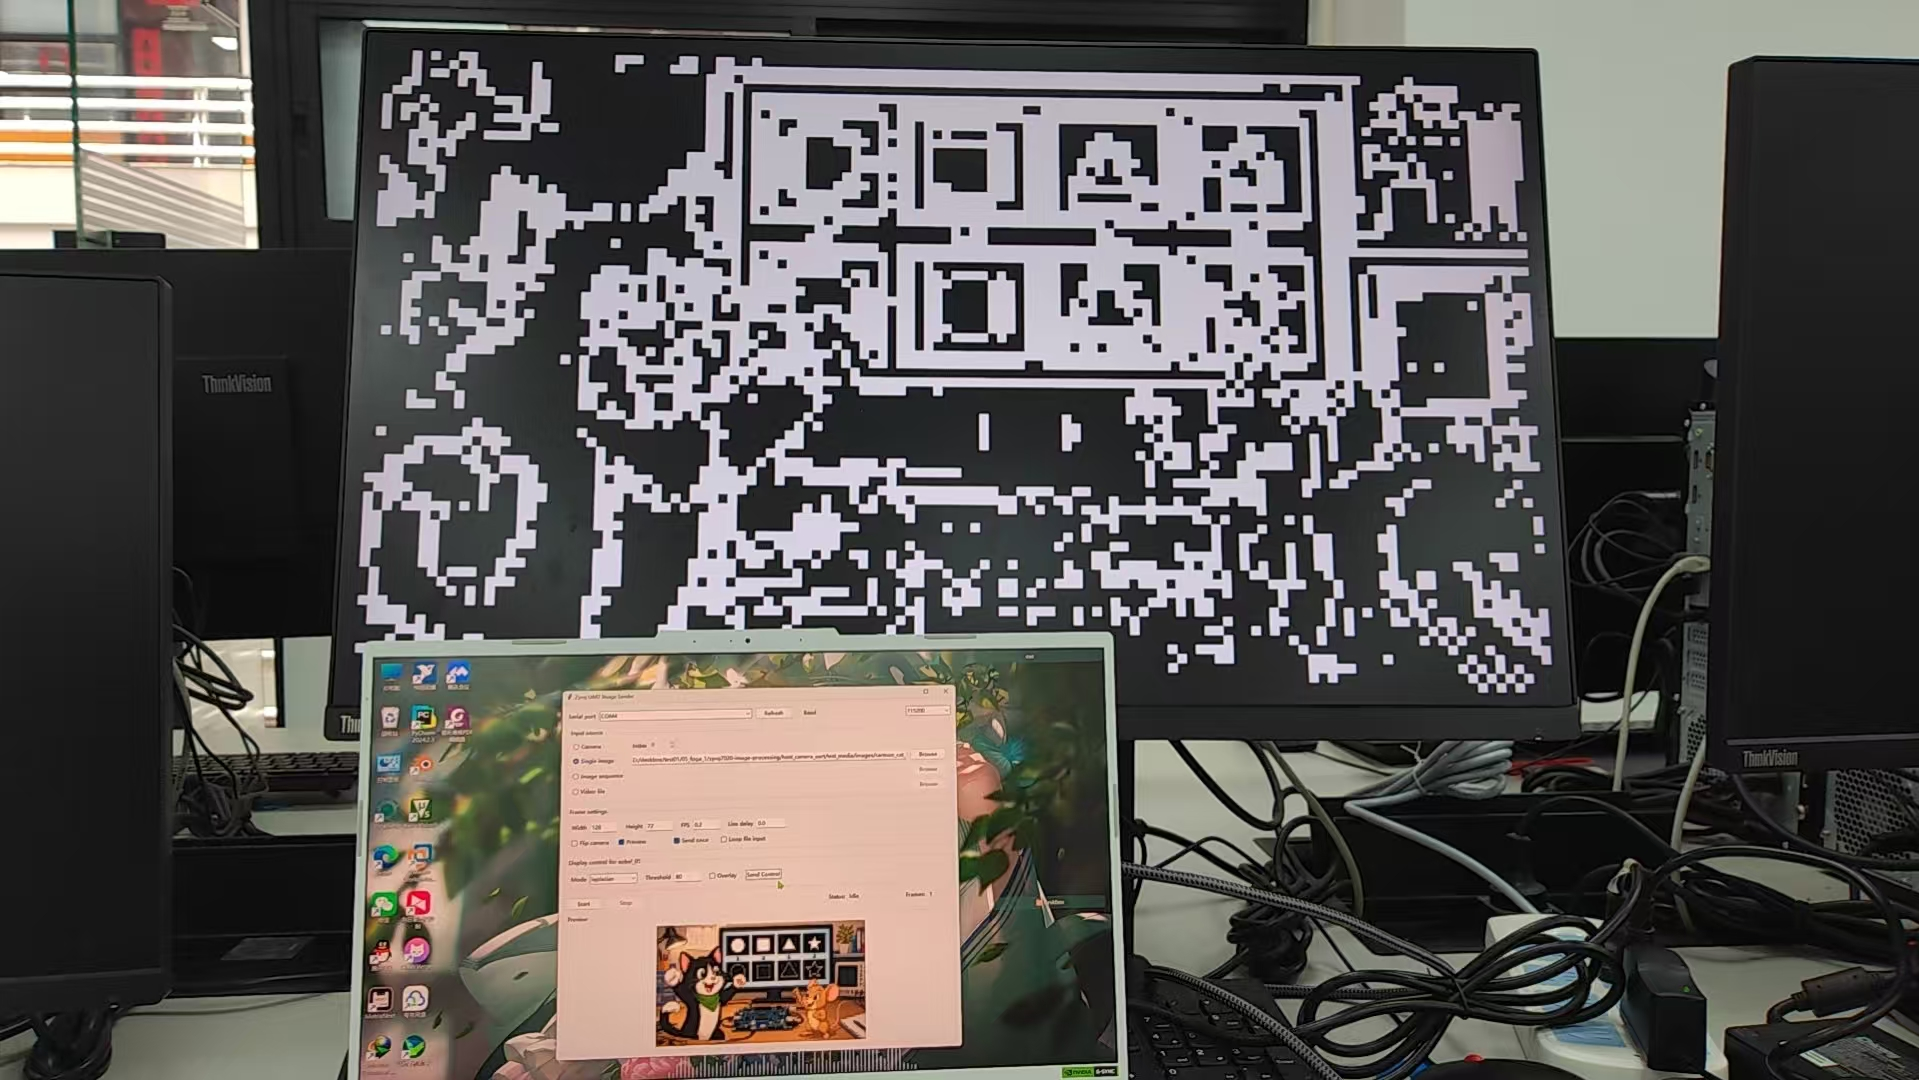
\includegraphics[width=\linewidth]{images/05扩展3/laplacian_80.jpg}
        \caption{Laplacian}
    \end{minipage}
    \hfill
    \begin{minipage}{0.48\textwidth}
        \centering
        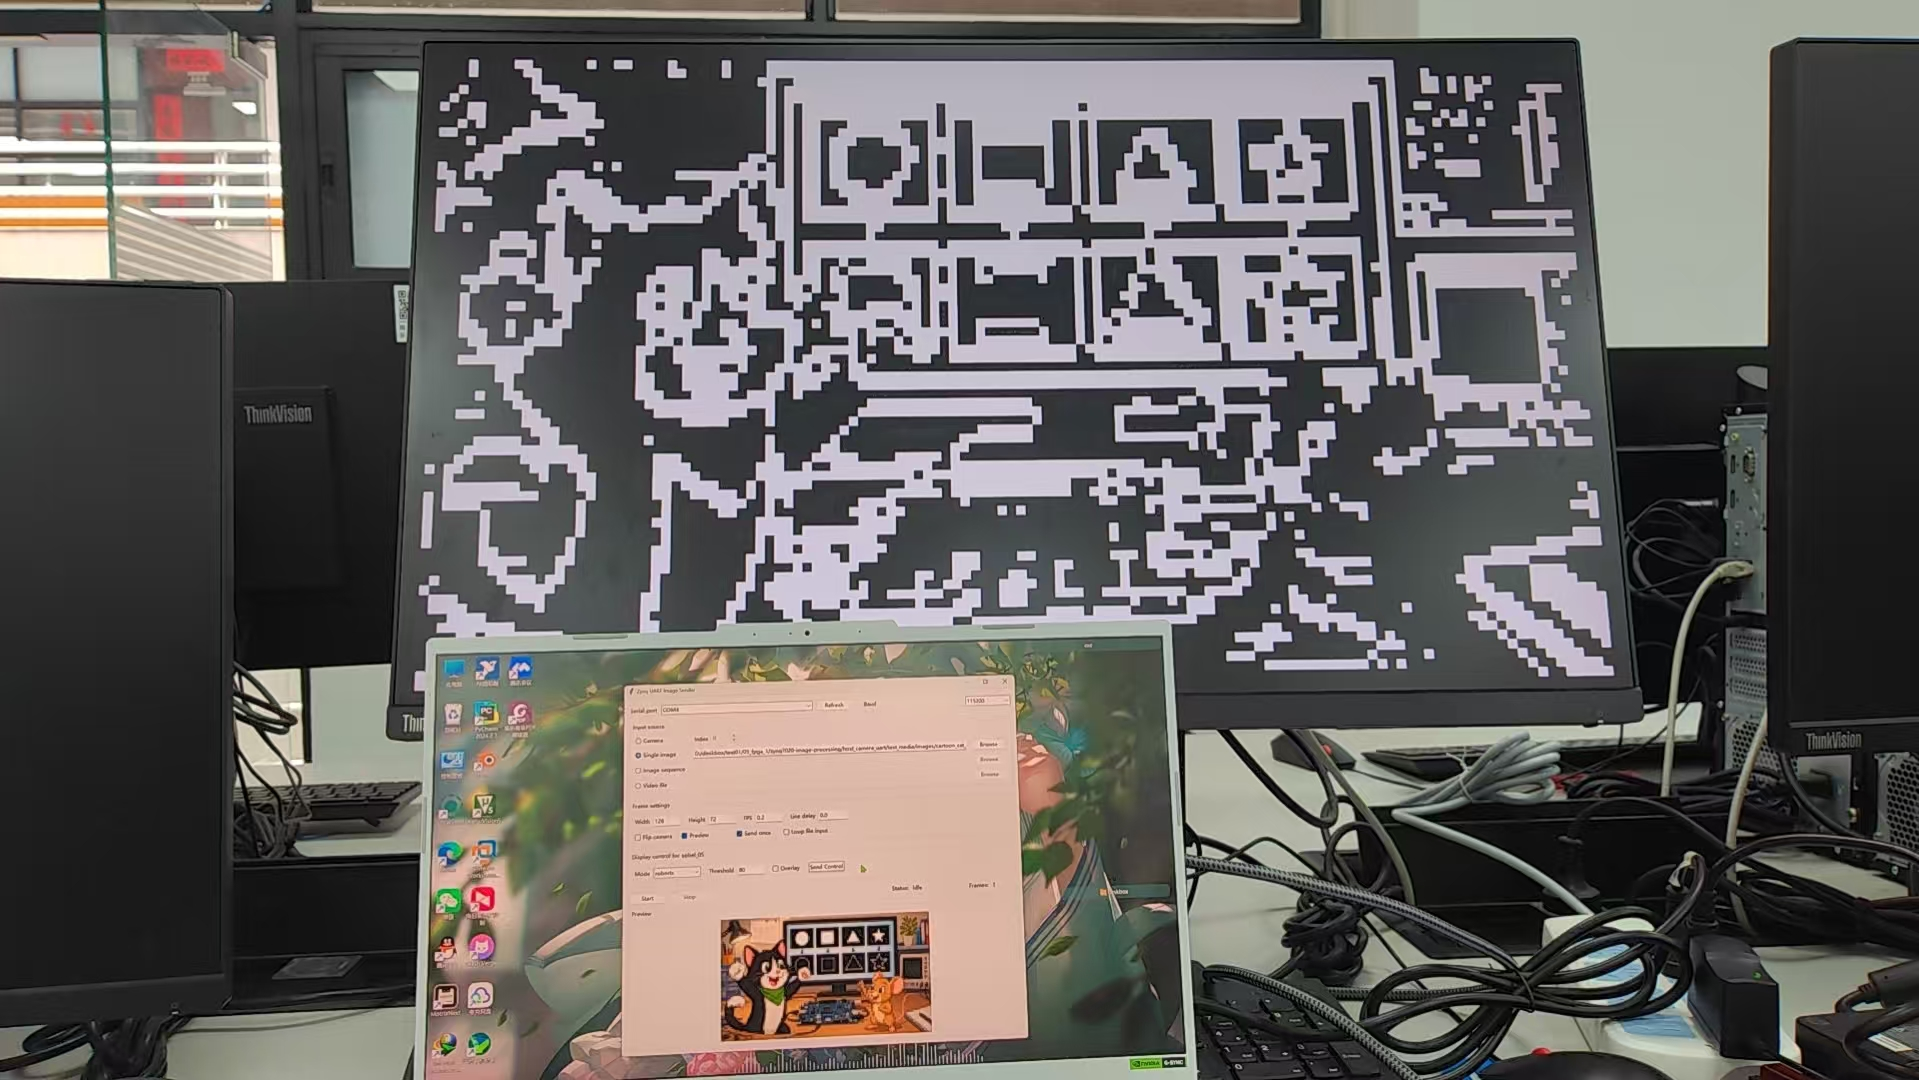
\includegraphics[width=\linewidth]{images/05扩展3/Robert_80.jpg}
        \caption{Roberts}
    \end{minipage}
    \caption{阈值80时四种算法对比}
    \label{fig:thresh80}
\end{figure}

如图\ref{fig:thresh80}所示，当阈值提高到80时，只有较强的边缘被保留。Sobel和Prewitt的边缘效果最为接近，Roberts保留了较多对角线边缘，Laplacian的边缘细节仍然最丰富。这表明在高阈值下，各算法的差异主要体现在边缘细节和噪声抑制上。

\subsubsection{资源利用率与时序结果}

Vivado综合后的资源利用率如图\ref{fig:resource}所示。新增3个算法核后，资源增量可控。Prewitt和Roberts由于不使用2x乘法，不消耗额外DSP资源；Laplacian的4倍乘法可优化为左移2位实现。四种算法共享行缓冲和灰度转换逻辑，资源利用率较高。

\begin{figure}[H]
    \centering
    
\includegraphics[width=0.9\textwidth]{images/05扩展3/资源利用率.png}
    \caption{Vivado资源利用率报告}
    \label{fig:resource}
\end{figure}

时序分析结果如图\ref{fig:timing}所示，新增三个算法模块后系统时序保持稳定，无时序违例。这得益于算法的并行架构设计，每个核独立处理，不会相互影响时序路径。

\begin{figure}[H]
    \centering
    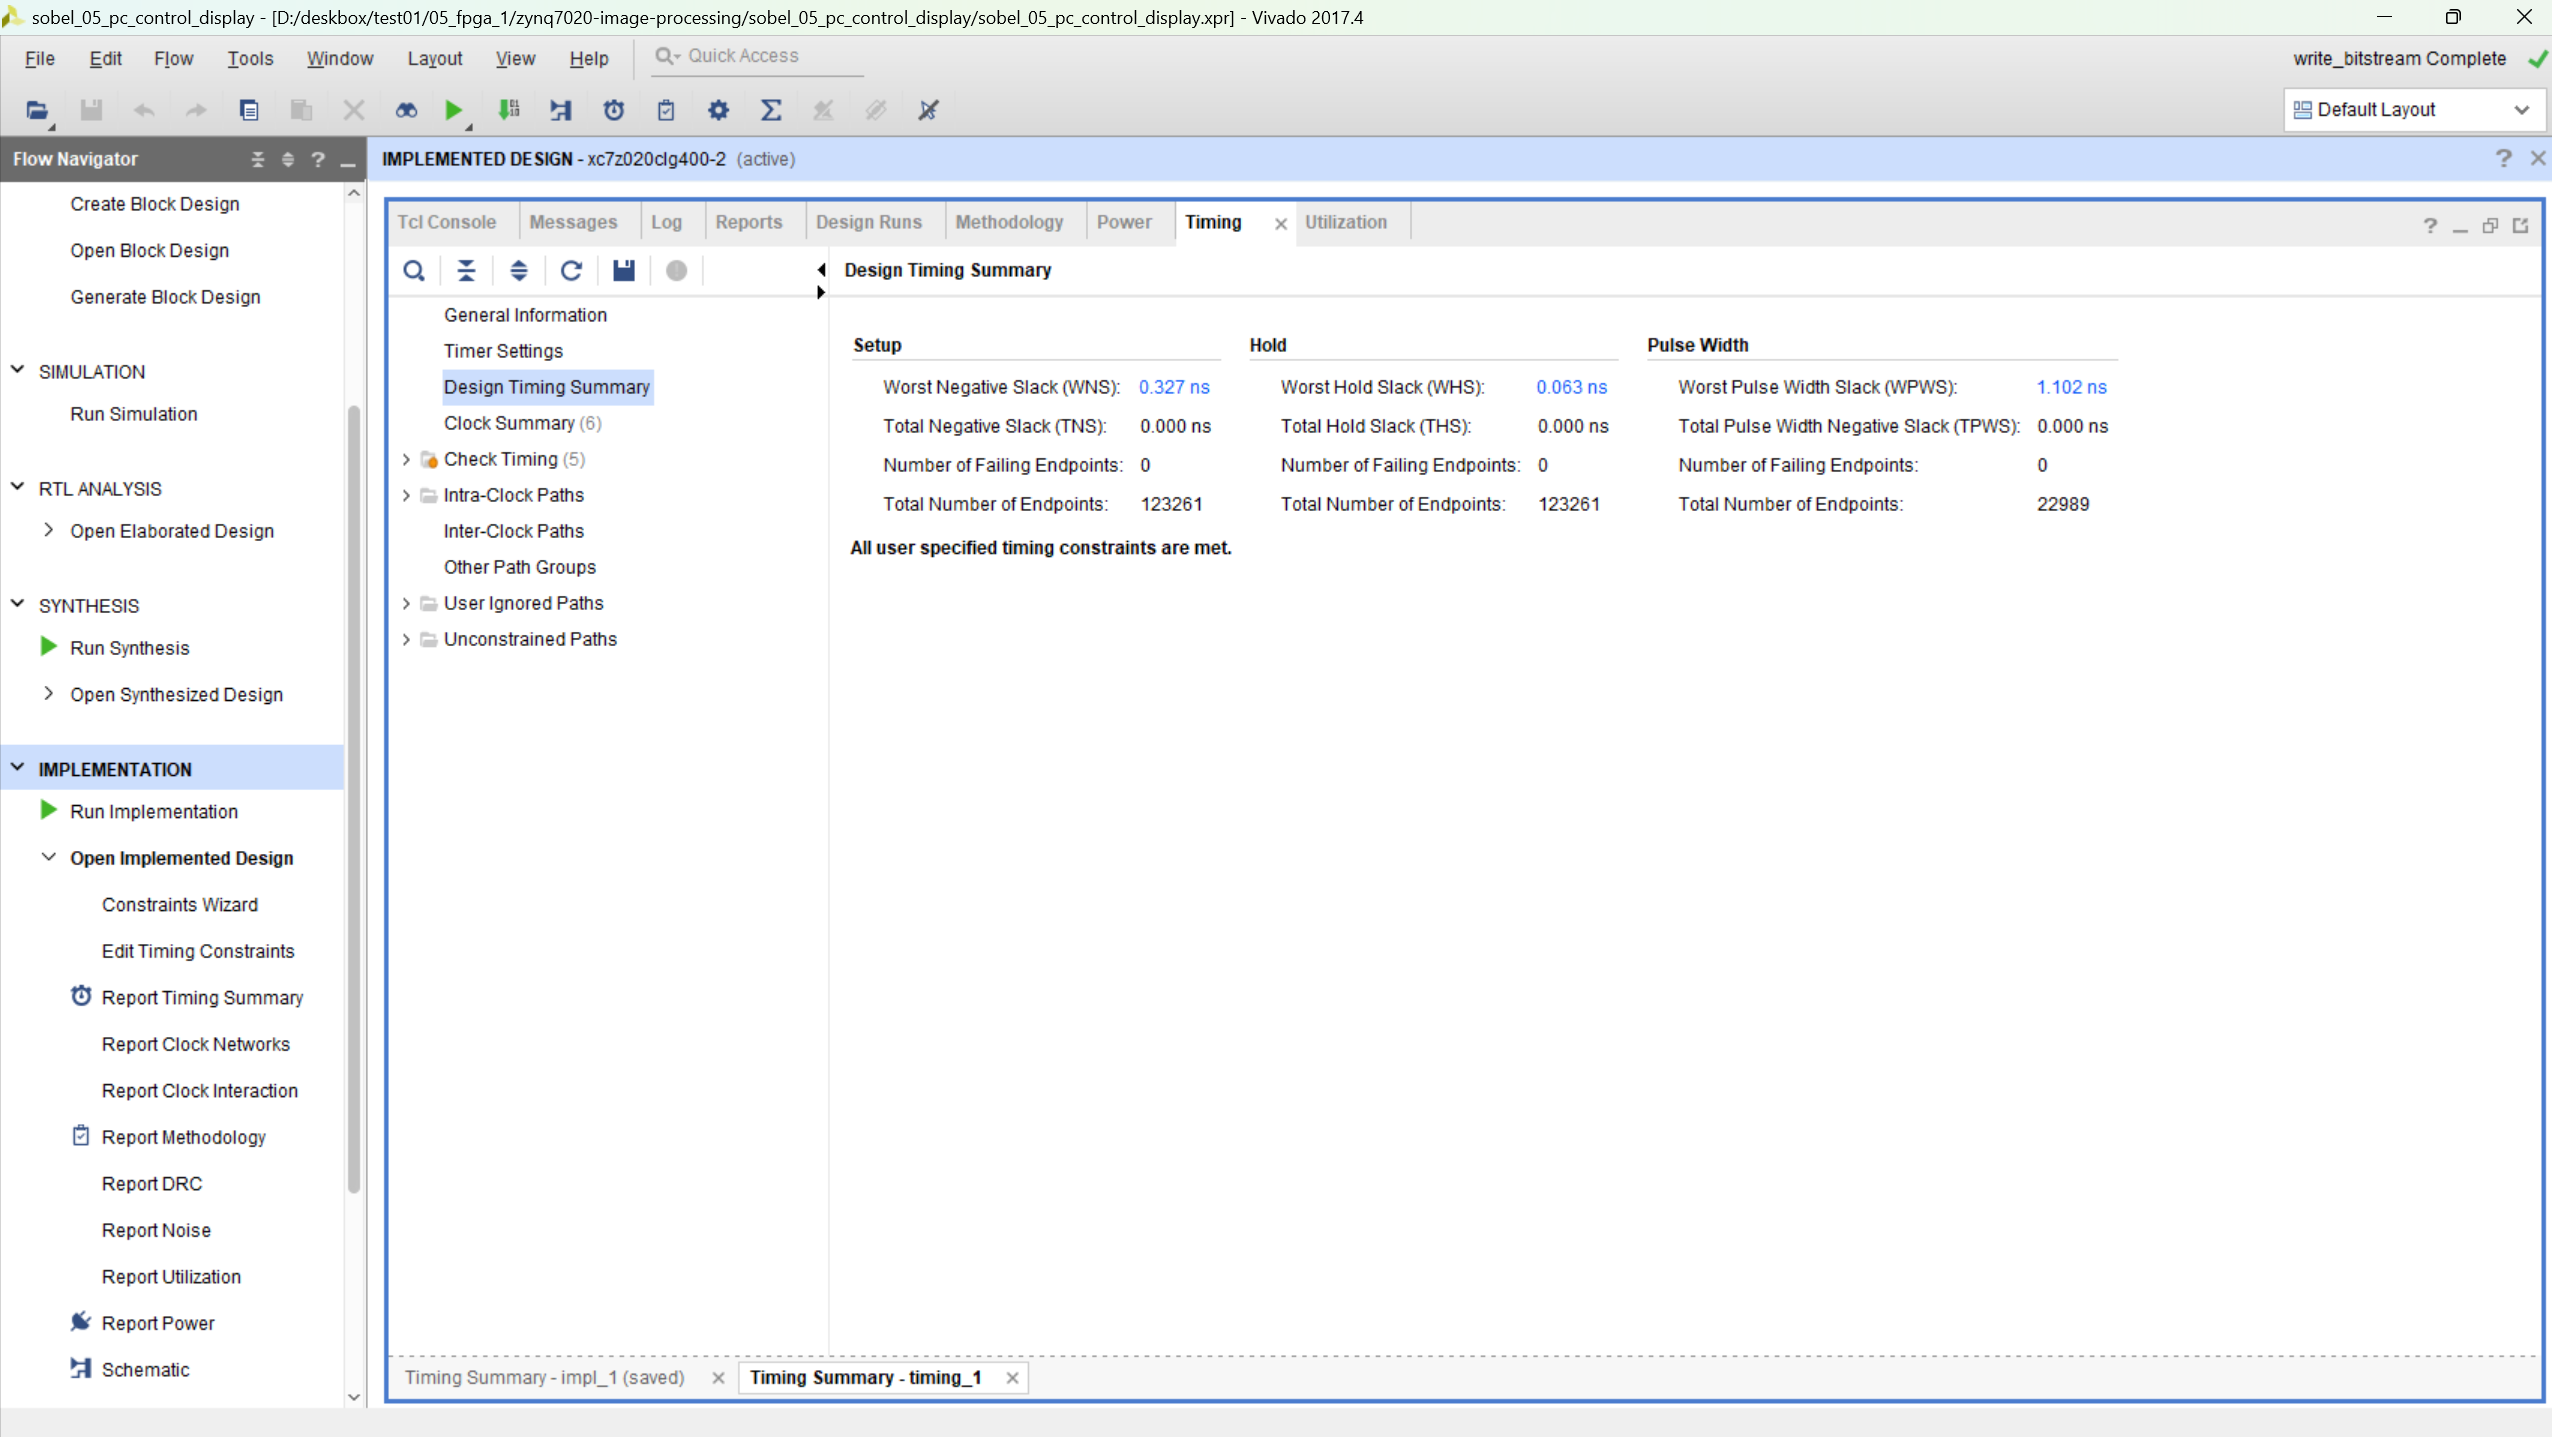
\includegraphics[width=0.9\textwidth]{images/05扩展3/时序对比分析.png}
    \caption{Vivado时序分析结果}
    \label{fig:timing}
\end{figure}

\subsubsection{上板演示现象}

上板验证结果如图\ref{fig:hw}所示，所有模式均可通过上位机命令实时切换。灰度图显示正确，Sobel边缘检测效果良好，彩色边缘叠加模式将原图与边缘叠加显示。

\begin{figure}[H]
    \centering
    \begin{minipage}{0.48\textwidth}
        \centering
        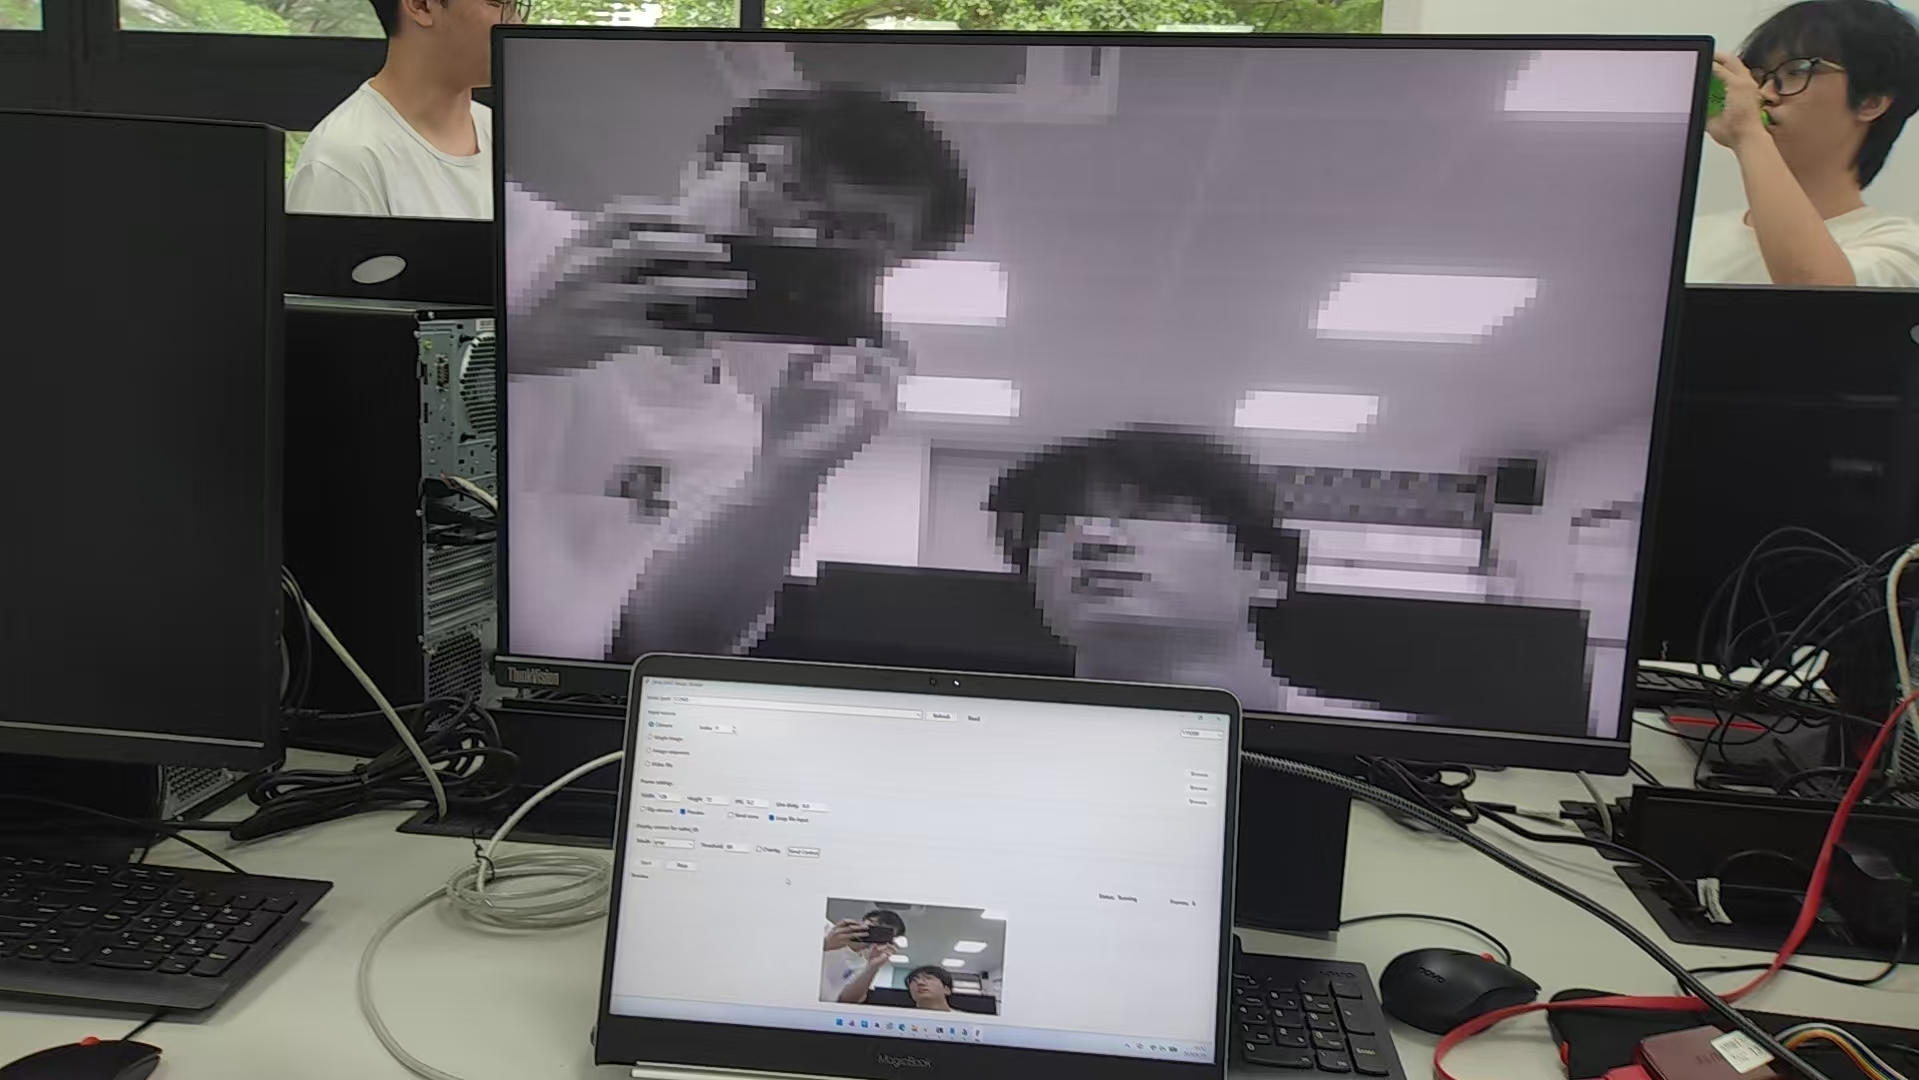
\includegraphics[width=\linewidth]{images/05/灰度图.jpg}
        \caption{灰度图显示}
    \end{minipage}
    \hfill
    \begin{minipage}{0.48\textwidth}
        \centering
        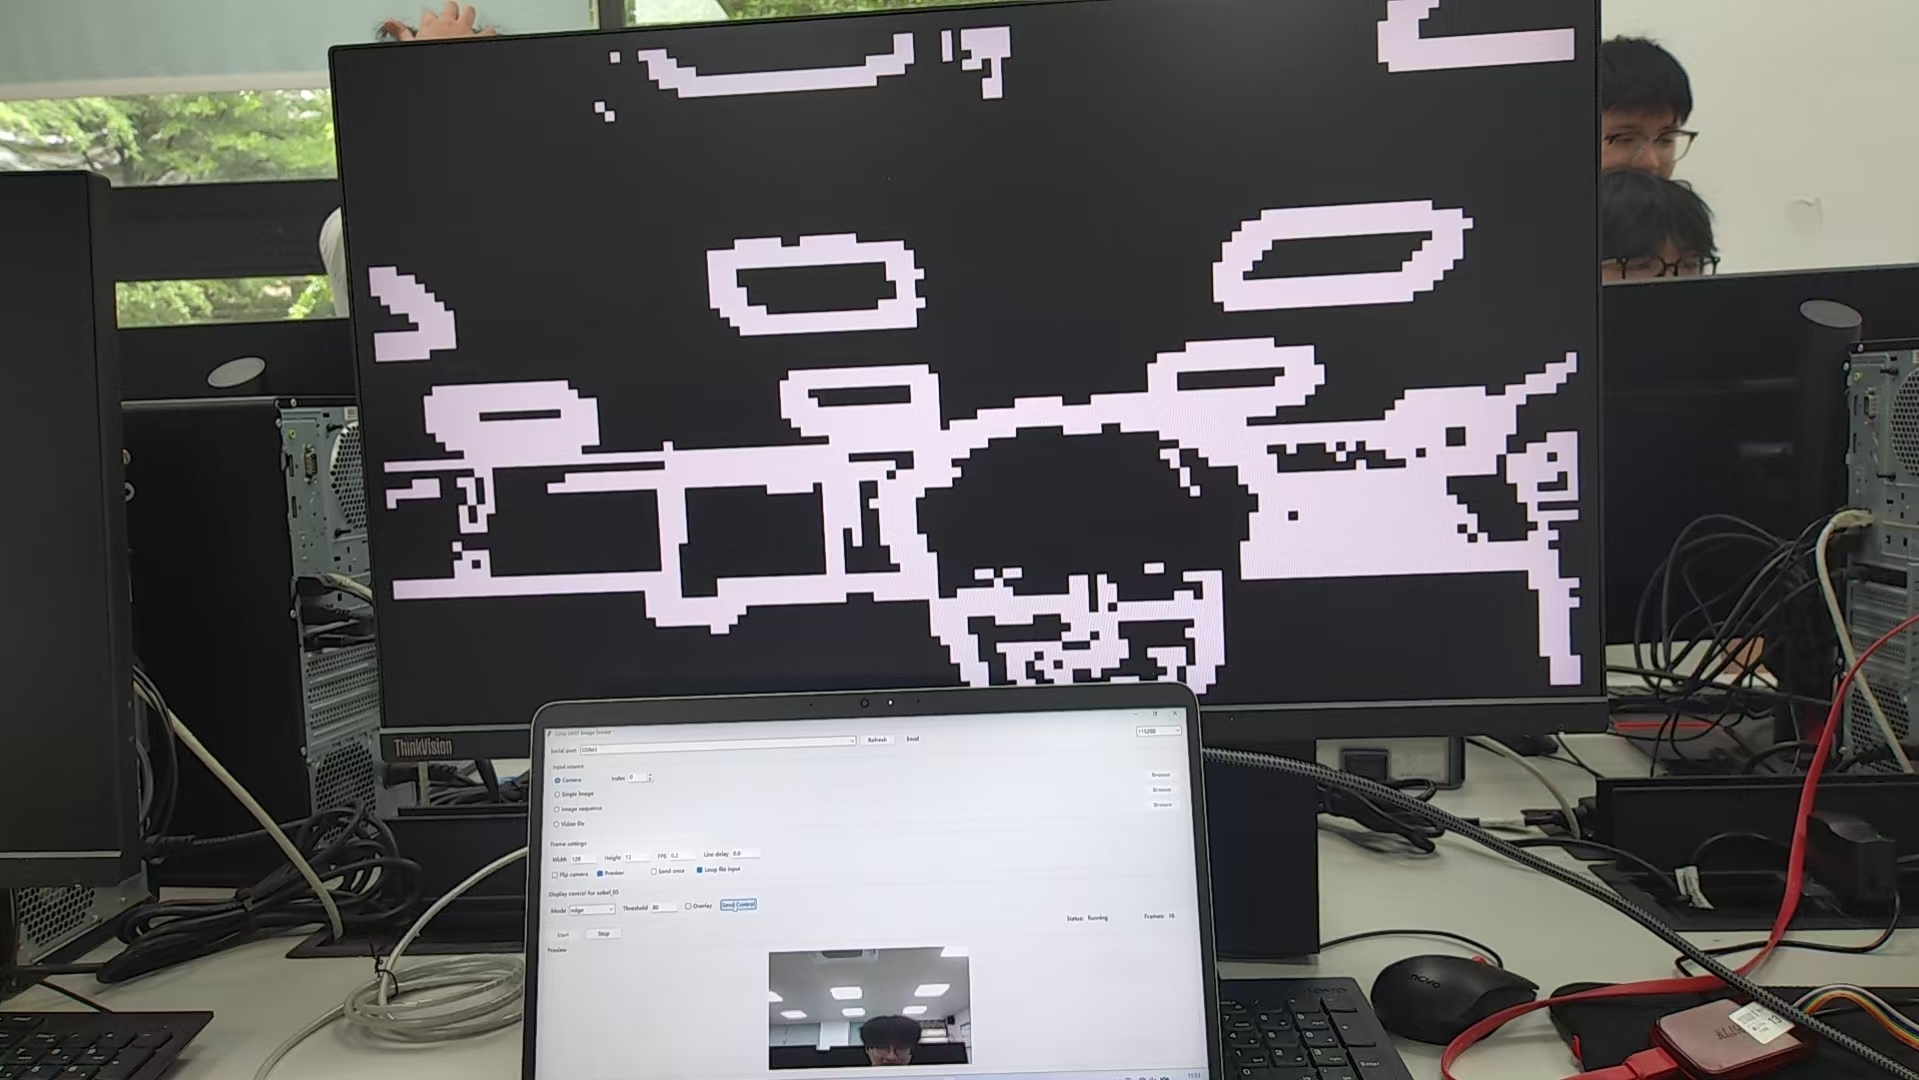
\includegraphics[width=\linewidth]{images/05/二值边缘图.jpg}
        \caption{Sobel边缘检测}
    \end{minipage}
    \par\vspace{1em}
    \begin{minipage}{0.48\textwidth}
        \centering
        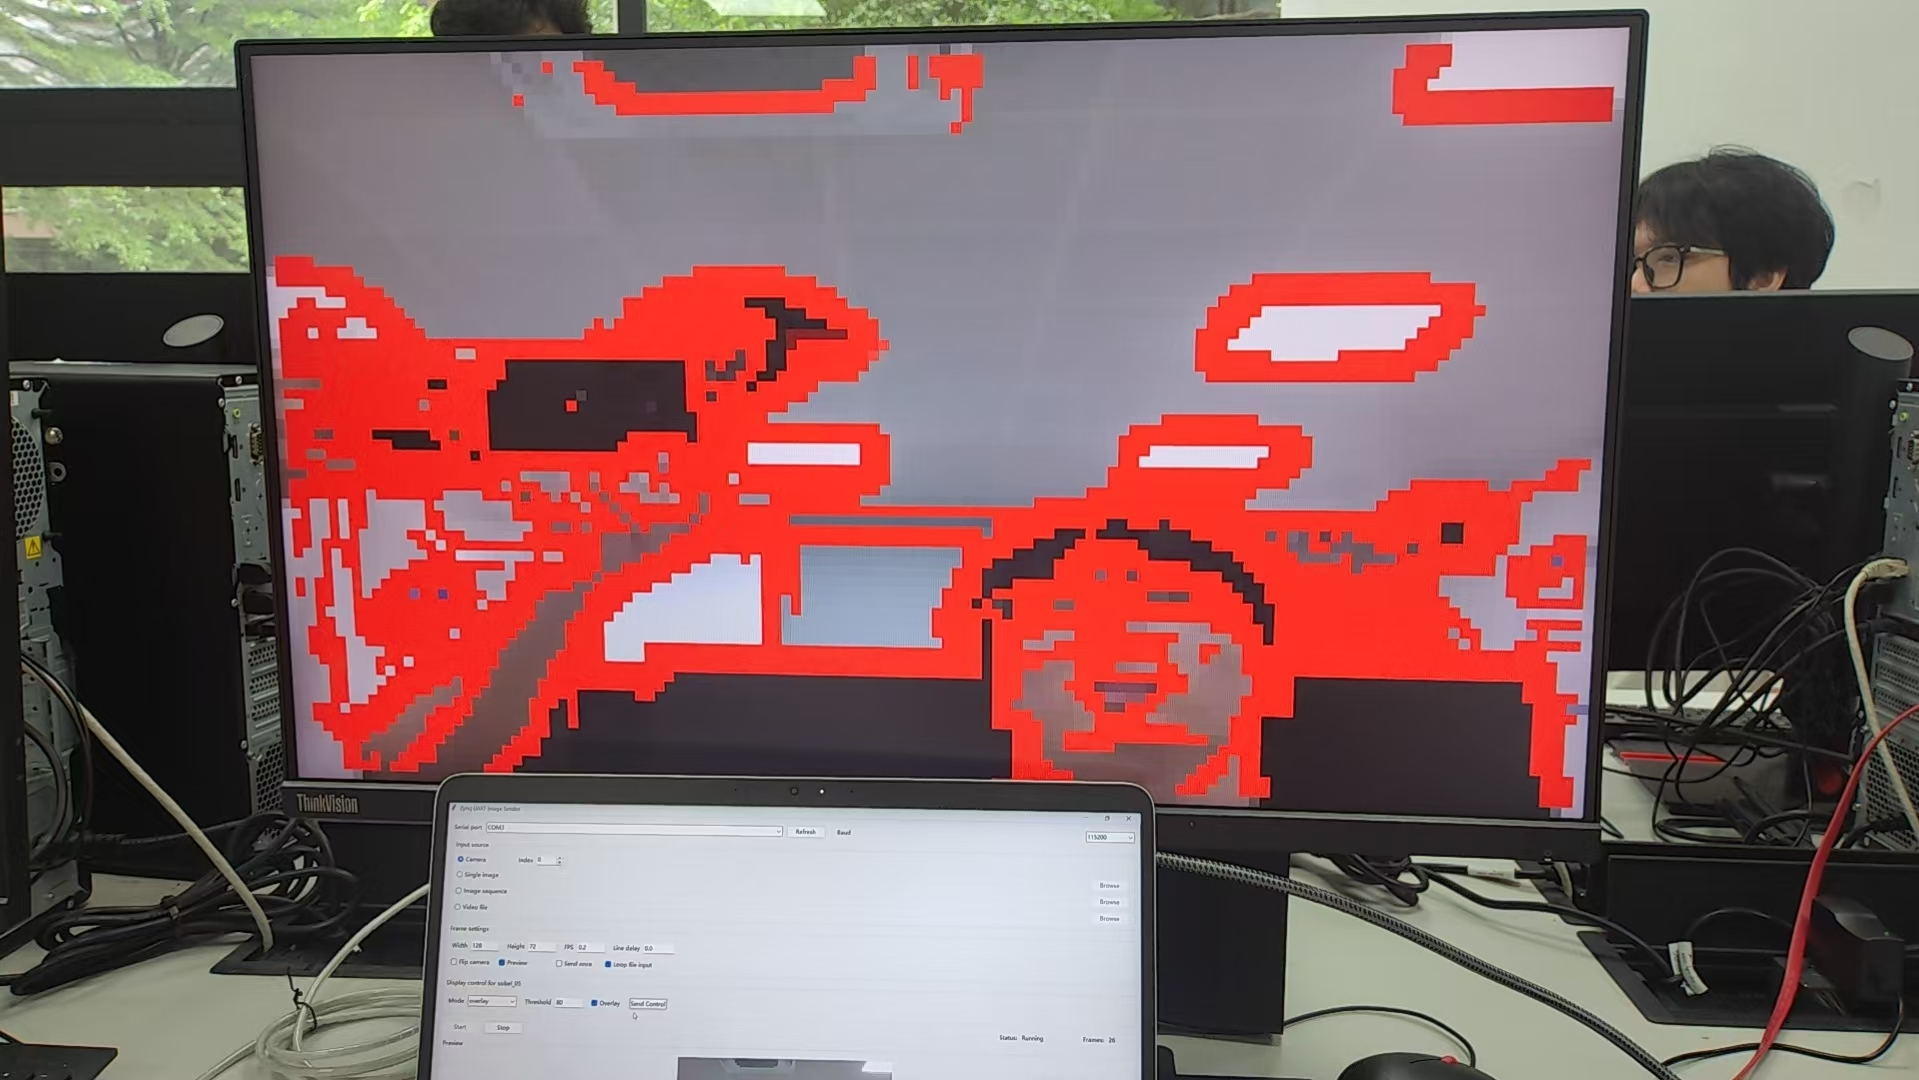
\includegraphics[width=\linewidth]{images/05/彩色边缘图.jpg}
        \caption{彩色边缘叠加}
    \end{minipage}
    \caption{上板验证结果}
    \label{fig:hw}
\end{figure}

\subsubsection{上位机控制界面}

上位机控制界面如图\ref{fig:ui}所示，支持模式切换和阈值调整。用户可通过命令A5 5A 01 04/05/06切换到Laplacian/Prewitt/Roberts模式，通过A5 5A 02 XX设置边缘二值化阈值。

\begin{figure}[H]
    \centering
    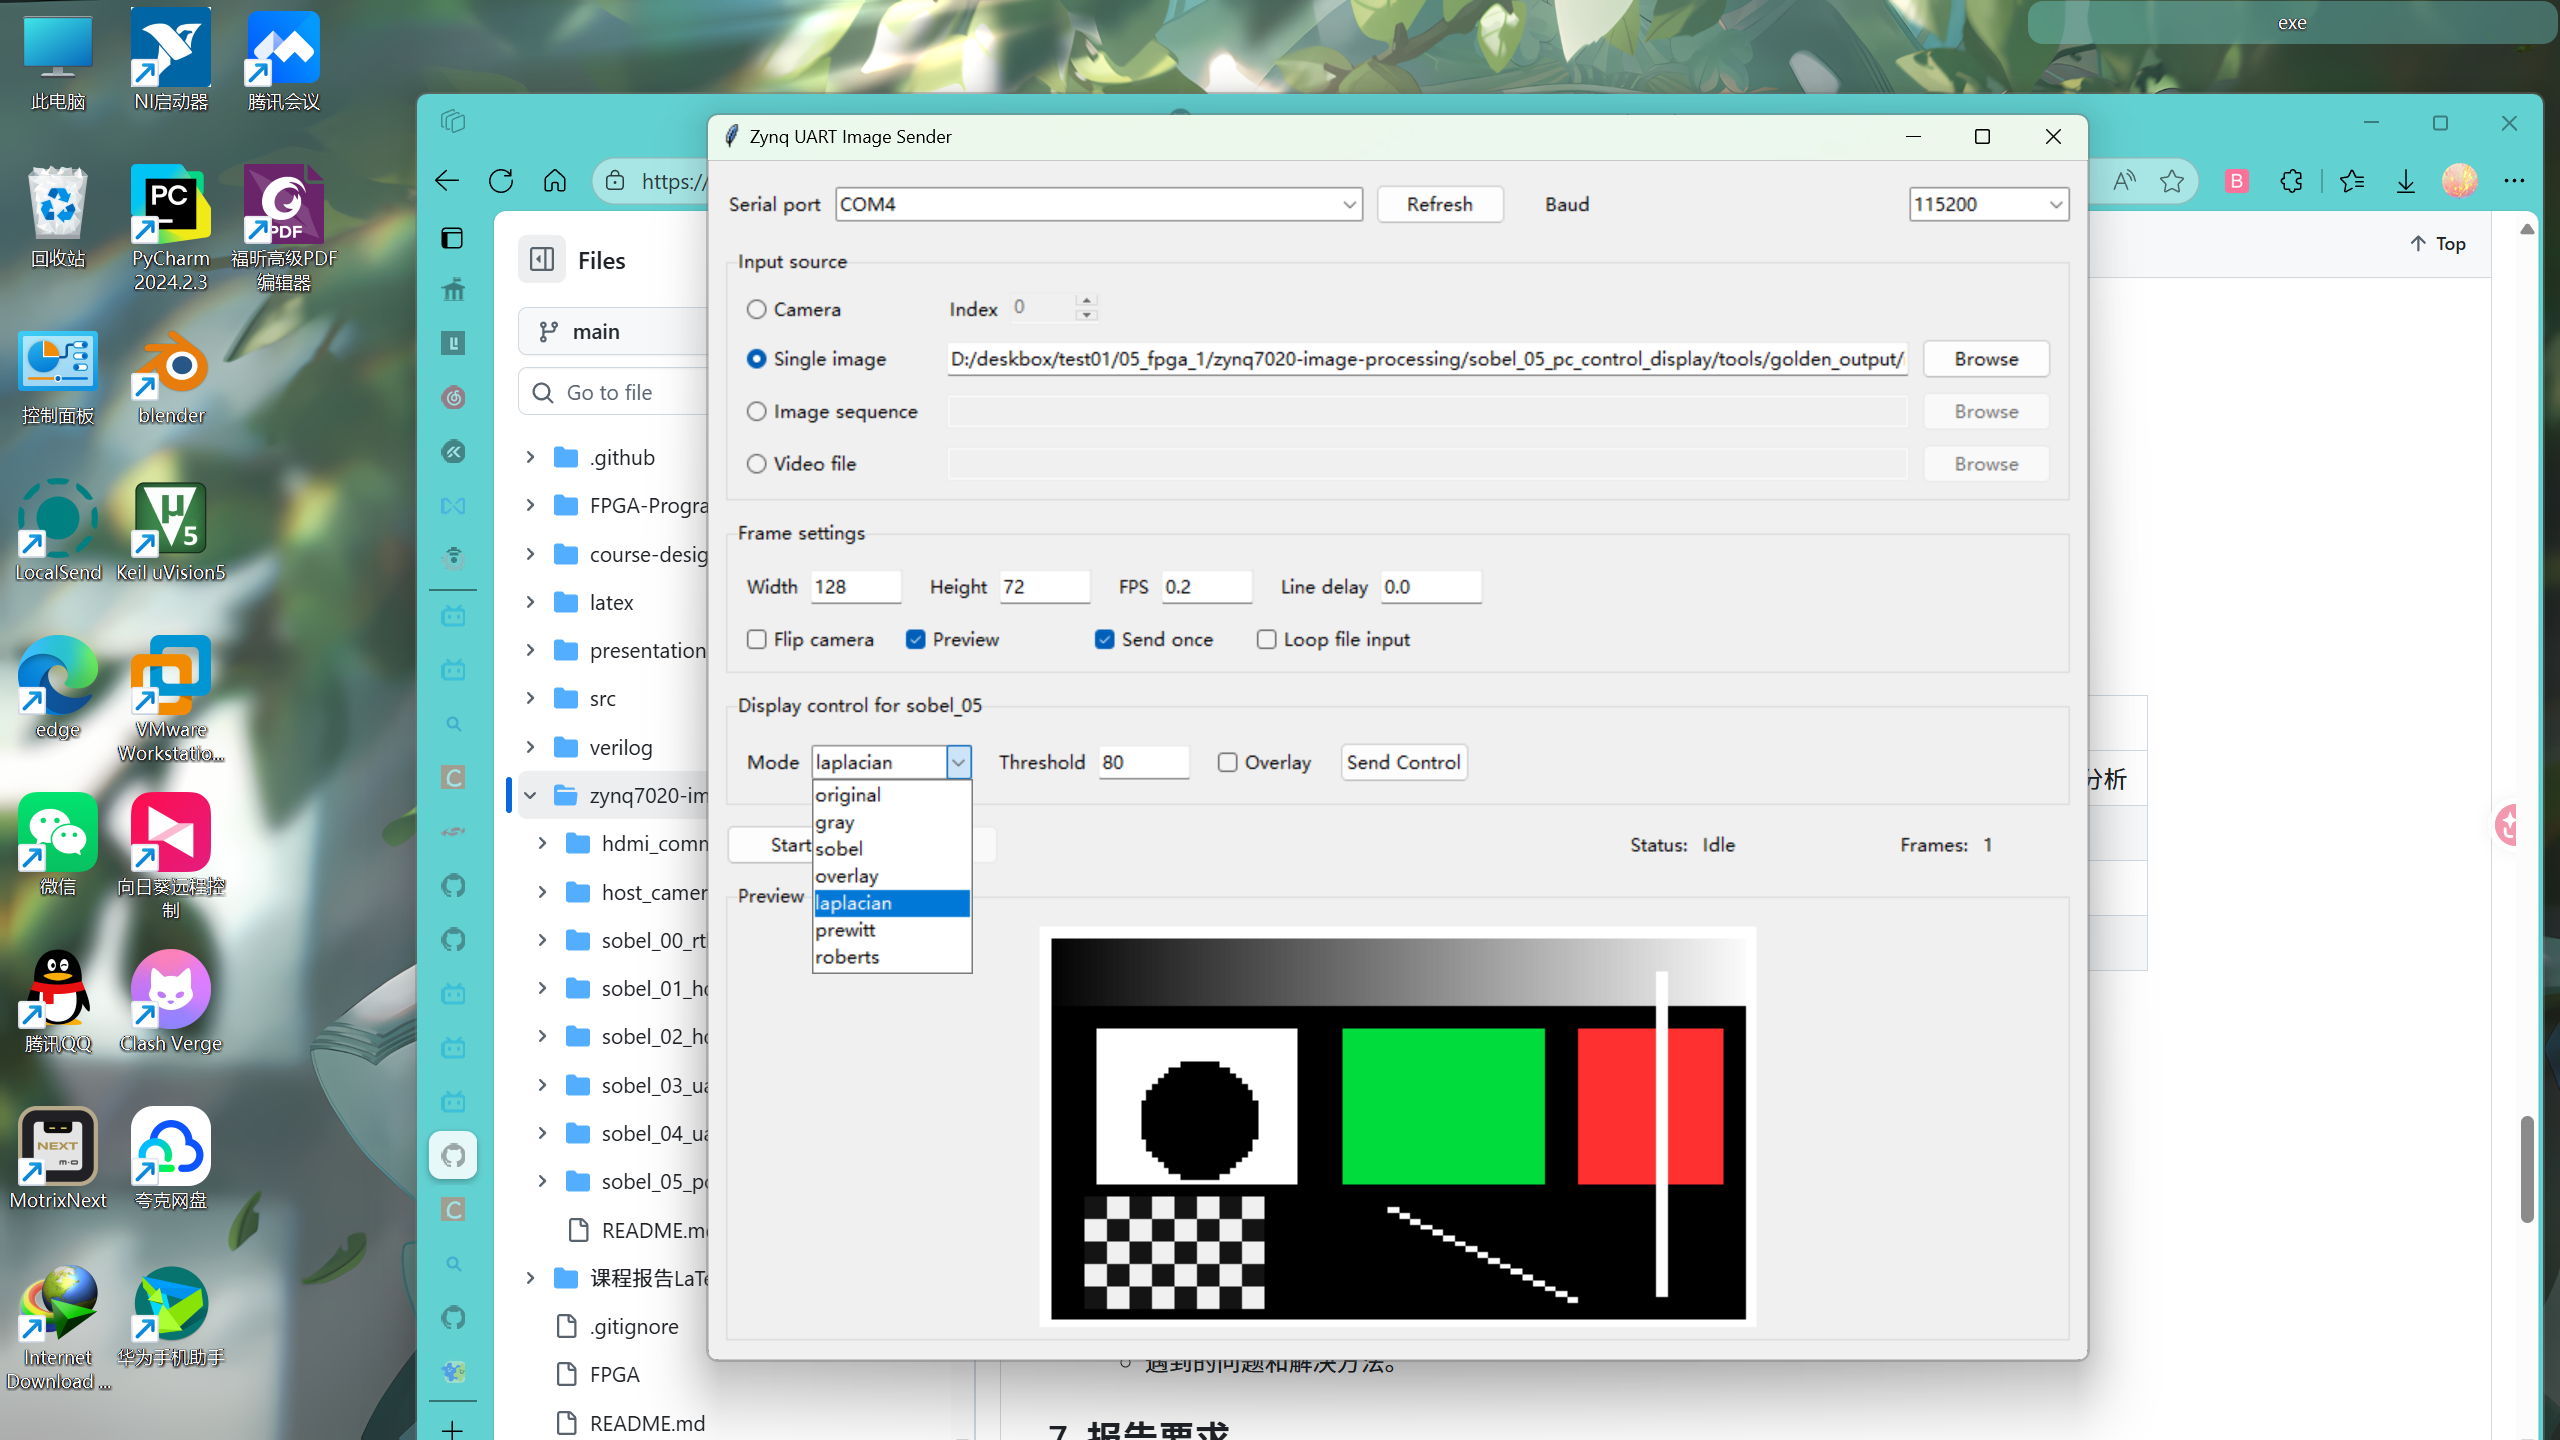
\includegraphics[width=0.9\textwidth]{images/05扩展3/上位机ui.png}
    \caption{上位机控制界面}
    \label{fig:ui}
\end{figure}

% !Mode:: "TeX:UTF-8"

\section{物料与成本}

\subsection{物料清单}

\begin{table}[h]
    \begin{tabular}{l|lll}
        \hline
        \multicolumn{1}{c|}{物料名称} & 数量   & 价格   & 用途   \\ \hline
        \multicolumn{1}{c|}{黑金ZYNQ7020开发板} & 1 & 约600元 & FPGA主控板 \\
        \multicolumn{1}{c|}{HDMI显示器} & 1 & 约800元 & 图像显示输出 \\
        \multicolumn{1}{c|}{USB串口线} & 1 & 约20元 & UART通信 \\
        \multicolumn{1}{c|}{HDMI线缆} & 1 & 约30元 & 显示连接 \\
        \multicolumn{1}{c|}{PC电脑} & 1 & 自备 & 上位机开发 \\
        \multicolumn{1}{c|}{电源适配器} & 1 & 约50元 & 开发板供电 \\ \hline
    \end{tabular}
\end{table}


\subsection{项目成本}

\begin{table}[h]
    \begin{tabular}{l|lll}
        \hline
        \multicolumn{1}{c|}{项目名称}  & 金额 & 说明 \\ \hline
        \multicolumn{1}{c|}{材料成本}  & 约1500元 & 开发板+显示器+线缆 \\
        \multicolumn{1}{c|}{工具和设备} & 约0元 & Vivado免费版+SDK \\
        \multicolumn{1}{c|}{其他费用}  & 约0元 & 无额外费用 \\ \hline
    \end{tabular}
\end{table}

\begin{itemize}
    \item 总成本预计: 约1500元（不含PC电脑）
\end{itemize}


\subsection{损耗与损坏}

本次实验过程中无物料损耗或损坏。所有硬件设备均正常工作，开发板、显示器和线缆均完好无损。

\subsection{主要物料图片展示}

\begin{figure}[h]
    \centering
    
\includegraphics[width=0.2\textwidth]{figures/logo.pdf}
    \caption{黑金ZYNQ7020开发板}
\end{figure}

% !Mode:: "TeX:UTF-8"

\section{个人贡献}


\subsection{报告撰写}

本实验报告由本人独立完成，包括：
\begin{itemize}
    \item 系统设计原理阐述
    \item 四种边缘检测算法原理分析
    \item 修改内容详解
    \item 仿真结果整理与分析
    \item 资源利用率和时序结果分析
    \item 实验现象记录与总结
\end{itemize}


\subsection{编码工作}

\begin{itemize}
    \item 参与prewitt\_core.v模块的代码编写和调试
    \item 参与laplacian\_core.v模块的代码编写和调试
    \item 参与roberts\_core.v模块的代码编写和调试
    \item 协助修改hdmi\_bram\_sobel\_display.v的模式扩展
    \item 参与仿真测试用例的编写
\end{itemize}

\subsection{硬件连接}

\begin{itemize}
    \item 负责ZYNQ7020开发板与HDMI显示器的连接
    \item 负责USB串口线与PC的连接调试
    \item 负责上板验证和现象记录
\end{itemize}

\subsection{资本投入}

本次实验主要使用实验室提供的设备，个人无额外资本投入。


\subsection{开发问题描述与解决方案}

\subsubsection{Prewitt边缘幅度较低}

\begin{itemize}
    \item 问题描述：Prewitt模式下边缘图整体较暗，细节不如Sobel清晰
    \item 解决方法：降低阈值补偿，或理解这是算法特性（无2x权重）
\end{itemize}



\subsubsection{Laplacian噪声敏感}

\begin{itemize}
    \item 问题描述：Laplacian对噪声敏感，边缘图噪点较多
    \item 解决方法：提高阈值过滤噪声，或理解这是二阶导数的特性
\end{itemize}



\subsubsection{Roberts边缘断裂}

\begin{itemize}
    \item 问题描述：Roberts使用2×2卷积核，边缘有时不连续
    \item 解决方法：降低阈值保留更多边缘，或理解这是小卷积核的限制
\end{itemize}



\subsubsection{模式切换命令格式}

\begin{itemize}
    \item 问题描述：新增模式4/5/6后，需要确保上位机命令格式正确
    \item 解决方法：参考现有命令格式，扩展3-bit模式支持
\end{itemize}



\subsubsection{仿真测试覆盖}

\begin{itemize}
    \item 问题描述：需要确保新增模式的仿真测试完整性
    \item 解决方法：新增4项算法专项测试，覆盖边界条件
\end{itemize}



\subsubsection{资源利用优化}

\begin{itemize}
    \item 问题描述：新增3个算法模块可能增加资源消耗
    \item 解决方法：Prewitt/Roberts不消耗额外DSP，Laplacian可优化为左移
\end{itemize}

% !Mode:: "TeX:UTF-8"

\section{项目成果与反思}

\subsection{成果展示}

本次扩展成功在sobel\_05\_pc\_control\_display基础上新增了Prewitt、Laplacian、Roberts三种边缘检测算法，主要成果：

\begin{itemize}
    \item 新增3个算法核心模块：prewitt\_core.v、laplacian\_core.v、roberts\_core.v
    \item hdmi\_bram\_sobel\_display.v扩展显示模式到3-bit，4种算法并行运行
    \item 仿真模型通过所有测试，覆盖7种显示模式的正确性验证
    \item Python golden output量化对比了4种算法差异
    \item 上位机命令A5 5A 01 04/05/06可切换Laplacian/Prewitt/Roberts模式
    \item 4个算法共享rgb\_to\_gray输出和BRAM scan流程，FPGA资源增量小
    \item Vivado综合通过，时序无违例，bitstream生成成功
    \item 上板验证成功，4种算法均可通过上位机命令实时切换
\end{itemize}

\subsection{项目评估}

\subsubsection{成功之处}

\begin{itemize}
    \item 算法实现高效：复用Sobel架构，仅修改卷积权重
    \item 并行处理设计：4个算法共享灰度转换，独立处理
    \item 完整的验证流程：RTL仿真 + Python参考 + 上板验证
    \item 资源利用合理：Prewitt/Roberts不消耗额外DSP资源
    \item 模式扩展成功：从4种模式扩展到7种，上位机兼容
    \item 所有验收项完成：仿真、资源、时序、上板演示
\end{itemize}

\subsubsection{不足之处}

\begin{itemize}
    \item 未实现左右分屏同时显示两种算法结果
    \item 各算法的彩色边缘叠加功能未实现
    \item 未实现多算法同时对比显示模式
    \item Laplacian噪声敏感问题未完全解决
\end{itemize}

\subsection{个人反思}

通过本次扩展任务，我深入理解了：

\begin{itemize}
    \item FPGA图像处理算法的硬件实现方法
    \item 不同边缘检测算子（一阶/二阶、不同卷积核大小）的特性和适用场景
    \item PS+PL协同设计的系统架构
    \item 从仿真到上板的完整验证流程
    \item 多算法并行处理的设计思路和资源优化方法
\end{itemize}

本项目展示了FPGA在图像处理领域的灵活性和高效性，成功实现了4种边缘检测算法的并行处理和实时切换，为后续更复杂的图像处理系统奠定了基础。

% !Mode:: "TeX:UTF-8"

\section{附录}

\subsection{完整代码附录}

注：个人代码贡献标注于 6.1 编码工作

核心模块prewitt\_core.v的关键代码如下：

\begin{lstlisting}[style=Verilog, title=\texttt{prewitt\_core.v 核心代码}]
// === Prewitt 卷积计算 ===
// 水平梯度Gx
gx = -$signed({4'd0, top0}) + $signed({4'd0, top2})
     - $signed({4'd0, mid0}) + $signed({4'd0, mid2})
     - $signed({4'd0, bot0}) + $signed({4'd0, bot2});

// 垂直梯度Gy
gy = -$signed({4'd0, top0}) - $signed({4'd0, top1}) - $signed({4'd0, top2})
     + $signed({4'd0, bot0}) + $signed({4'd0, bot1}) + $signed({4'd0, bot2});

// 边缘强度 = |Gx| + |Gy|
mag = abs_gx + abs_gy;
edge_data <= (mag > 8'd255) ? 8'd255 : mag[7:0];
\end{lstlisting}

核心模块laplacian\_core.v的关键代码如下：

\begin{lstlisting}[style=Verilog, title=\texttt{laplacian\_core.v 核心代码}]
// === Laplacian 二阶导数计算 ===
// 4-邻域卷积核: [0 -1 0; -1 4 -1; 0 -1 0]
// L = 4*mid1 - top1 - mid0 - mid2 - bot1
laplace = ($signed({4'd0, mid1}) <<< 2)
         - $signed({4'd0, top1})
         - $signed({4'd0, mid0})
         - $signed({4'd0, mid2})
         - $signed({4'd0, bot1});

// 取绝对值
abs_laplace = laplace[10] ? (~laplace + 11'd1) : laplace;

// 边缘输出
edge_data <= (abs_laplace > 11'd255) ? 8'hff : abs_laplace[7:0];
\end{lstlisting}

核心模块roberts\_core.v的关键代码如下：

\begin{lstlisting}[style=Verilog, title=\texttt{roberts\_core.v 核心代码}]
// === Roberts Cross 对角线梯度计算 ===
// 2×2卷积核
// Gx = top_left - bottom_right
// Gy = top_right - bottom_left
gx = $signed({2'd0, top_left}) - $signed({2'd0, bottom_right});
gy = $signed({2'd0, top_right}) - $signed({2'd0, bottom_left});

// 取绝对值
abs_gx = gx[9] ? (~gx + 10'd1) : gx;
abs_gy = gy[9] ? (~gy + 10'd1) : gy;

// 边缘强度 = |Gx| + |Gy|
mag = abs_gx + abs_gy;
edge_data <= (mag > 11'd255) ? 8'hff : mag[7:0];
\end{lstlisting}

\subsection{文件修改对照表}

\begin{table}[h]
    \centering
    \begin{tabular}{|c|c|c|}
        \hline
        文件 & 操作 & 说明 \\
        \hline
        prewitt\_core.v & 新增 & Prewitt边缘检测核心模块 \\
        \hline
        laplacian\_core.v & 新增 & Laplacian边缘检测核心模块 \\
        \hline
        roberts\_core.v & 新增 & Roberts边缘检测核心模块 \\
        \hline
        hdmi\_bram\_sobel\_display.v & 修改 & 集成3个算法核 + 模式4/5/6 + 3-bit扩展 \\
        \hline
        sim/display\_control\_model.v & 修改 & 支持MODE\_LAPLACIAN/PREWITT/ROBERTS \\
        \hline
        sim/display\_control\_model\_tb.v & 修改 & 新增算法测试用例 \\
        \hline
        ps\_uart\_control\_bram\_app/src/main.c & 修改 & mode位掩码扩展到0x07 \\
        \hline
    \end{tabular}
    \caption{文件修改对照表}
    \label{tab:file_changes}
\end{table}

\clearpage
\section{参考资料、文献}
\begin{enumerate}
    \item 王金明. 数字系统设计与Verilog HDL(第7版). 电子工业出版社, 2019.
    \item Xilinx. Zynq-7000 SoC Technical Reference Manual, 2021.
    \item Gonzalez, R.C. Digital Image Processing. Pearson, 2018.
    \item 实验05扩展报告\_Prewitt边缘检测算法集成.
\end{enumerate}


% 附录
\appendix
\section{\centering 设计图纸}
\subsection*{系统架构图}
完整系统架构图见附件。

\section{\centering 代码清单}
完整Verilog源代码见随附文件。

\end{document}
